\documentclass[12pt]{report}			% Začátek dokumentu
\usepackage{SP}							% Import stylu

\author{Jonáš Havelka}
\title{Neuronová síť}
\date{19. února 2020}
\vedouci{Dr. rer. nat. Michal Kočer}
\place{V Českých Budějovicích}
\skolnirok{2019/2020}
\logo{
\includegraphics[scale=0.75]{logo_gymji.jpg}}

\newcommand{\Kotlin}{\icon{Kotlin-logo.png}\gls{Kotlin}}
\newcommand{\git}{\underlineicon{Git-logo.png}\,git}
\newcommand{\GitHub}{\bigunderlineicon{GitHub-logo.png}\,GitHub}
\newcommand{\Gradle}{\bigicon{Gradle-logo.png}Gradle}

\newcommand{\R}{\mathbb{R}}   			% množina reálnách čísel
\newcommand{\Z}{\mathbb{Z}}   			% množina celých čísel
\newcommand{\N}{\mathbb{N}}   			% množina přirozených čísel
\newcommand{\powerset}[1]{\mathcal{P} ( #1 )}   
										% potenční množina -- množina všech podmnožin
										
\usepackage{fancyvrb}					% balíček pro použití verbatim v poznámkách pod čarou
\usepackage{subcaption}					% balíček pro figuru s více obrázky
\VerbatimFootnotes

\begin{document}

	\mytitlepage						% Vygenerování titulní strany
	
	\prohlaseni{
		Prohlašuji, že jsem tuto práci vypracoval samostatně s vyznačením všech použitých pramenů.
	}	
	
	\abstrakt{
	
		Neuronové sítě se dnes objevují všude, ať už jde o vyhledávání, překládání nebo třeba jen zpracovávání dat. Mnoho programovacích jazyků má své knihovny pro práci s umělou inteligencí, ale zrovna \Kotlin{}, který je mým oblíbeným programovacím jazykem a lze použít skoro kdekoliv (webové stránky, servery, mobily), takovou knihovnu postrádá. Proto jsem se rozhodl svoji práci koncipovat jako snahu o implementování takové knihovny.
		% Abstrakt
	}{
		Neuronové sítě, \Kotlin, Umělá inteligence, Multiplatformní knihovna						% Klíčová slova
	}
	
	\podekovani{
		Poděkování patří hlavně mému učiteli informatiky, který je zároveň vedoucím mé práce, za skvělou výuku na hodinách a velkou trpělivost při kontrole našich prací. Také nesmím zapomenout na Alžbětu Neubauerovou, která mě celý rok podporovala a několikrát provedla korekturu mé práce.
		
		Dále bych rád poděkoval všem komunitám, jejichž nástroje jsem používal, tj.~\mbox{JetBrains}, v jejichž programovacím jazyce \Kotlin{} programuji a jejichž prostředí IntelliJ k tomu využívám, \Gradle{}, který používám ke kompilaci, \LaTeX{}, ve kterém píšu text a dále \git{} a~\GitHub{}, jež uchovávají má data, ať už text nebo knihovnu. 					% Poděkování
	}
	
	\tableofcontents\newpage			% Obsah
	
	
	
	
	\chapter*{Úvod}
	
		Neuronové sítě jsou v poslední době velmi skloňované téma. Nikdo vlastně pořádně neví, jak to, že fungují tak dobře, avšak cílem této práce však nebude zkoumat neuronové sítě, ale implementovat je v co největším rozsahu (ať už struktury bez širšího využití jako asociativní paměť nebo často používané konvoluční sítě na rozpoznávání obrázků).
		
		Kotlin je ideální programovací jazyk pro vývoj knihovny, protože umožňuje tuto knihovnu používat jak pro \gls{JVM}, tak i v prohlížeči nebo v programech kompilovaných přímo do binárního kódu.
		
		Celá maturitní práce je k dispozici na GitHubu, text včetně zdrojového LaTeXu na adrese \url{https://github.com/JoHavel/Maturitni-Seminarni-Prace/tree/my\_work} a knihovna samotná pak na \url{https://github.com/JoHavel/NeuralNetwork}.
	
	
	\part{Teoretická část}
		
			\chapter{Laický náhled na neuronové sítě}
			
				\section{Neuron}
					Počítačové neuronové sítě nejsou jen výmysl lidí, jejich základ nalezneme v~nervových soustavách živočichů. Základní stavební jednotka takové soustavy (stejně tak i neuronové sítě) je neuron. Neuron funguje tak, že přes \gls{dendrit}y přijímá elektrické (přesněji iontové) signály od jiných neuronů a když součet signálů přeteče určitou danou mez, vyšle neuron signál přes \gls{axon}y dál do dalších neuronů.
					
					Přenos signálu z \gls{axon}u do \gls{dendrit}u se odehrává v malých prostorách mezi nimi zvaných \gls{synapse}. Vodivost synapsí je ovlivněna jejich chemickým složením, a proto se domníváme, že proces učení probíhá měněním těchto chemických spojů \autocite[s. 491]{Book:Informatika}.
					
					Náš umělý neuron tedy bude mít seznam \gls{dendrit}ů (nesoucích informaci z jakého neuronu vedou signál a jak ho mění \gls{synapse}), tzv. aktivační funkci (viz dále) a výstupní signál. Často navíc bude obsahovat základní hodnotu (angl. bias), která reprezentuje hladinu iontů v neuronu (v podstatě posouvá aktivační funkci ve směru osy $x$).
					
					\begin{figure}
						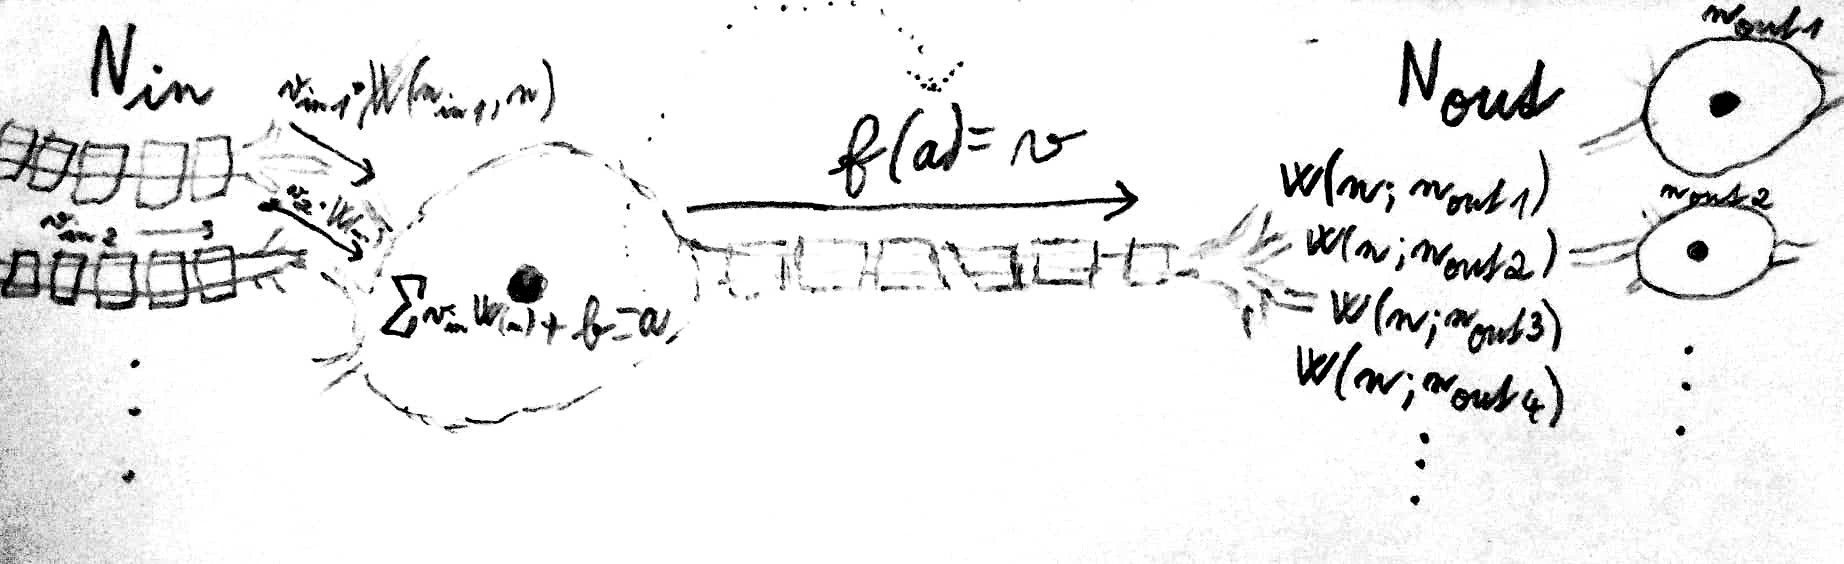
\includegraphics[width=\textwidth]{neuron}
						\caption{Analogie umělého a biologického neuronu.}
						\label{fig:neuron}
					\end{figure}
				
				\section{Aktivační funkce}
					Jak už bylo zmíněno, přírodní neuron funguje na principu toho, že když součet vstupních signálů nepřekračuje určitou mez, nevysílá neuron žádný (nebo téměř žádný) signál. Když je však tato mez překonána, neuron vyšle signál. V podstatě tedy vysílá buď 0 nebo 1. Pro účely umělého neuronu je 0 a 1 nedostačující, jelikož při procesu učení potřebujeme měnit hodnoty jemně, abychom nerozbili předchozí znalosti.
					
					Proto se jako aktivační funkce (tedy to, co určuje jaký má být výstup v závislosti na součtu vstupů, v případě přírody tedy funkce zobrazující interval $-\infty$ až mez na 0 a zbytek na 1 TODO(tohle přepsat)) používají funkce co nejvíce podobné právě tomuto binárnímu kroku, které jsou ale spojité a mají co \uv{nejhezčí} derivace (protože při zpětné propagaci právě podle derivace určíme, jak moc daný neuron ovlivňuje výsledek).
				
				\section{Sítě}
					Jelikož nahodilé neurony by se těžko udržovaly v paměti a operace na nich by byly velmi pomalé, potřebujeme síť nějak uspořádat. Nejjednodušším uspořádáním jsou vrstvy. Každý neuron z nějaké vrstvy má \gls{dendrit}y ze všech neuronů z vrstvy minulé. Tak se předejde cyklům, které jsou složité na výpočty, a navíc si nemusíme u každého neuronu pamatovat, ze kterých neuronů do něj vede signál.
					
				\section{Dopředná propagace a zpětná propagace}
					Dopředná propagace (častěji se používá anglický výraz forward propagation) je jednoduše spočítání signálů ve všech neuronech. Tedy u každého neuronu se sečtou vstupní signály (popř. přičte bias) a spočítá se funkční hodnota aktivační funkce v tomto bodě.
					
					Naopak zpětná propagace (častěji se používá anglický výraz backward propagation či backpropagation) je na základě chyby, kterou spočítáme z výstupu neuronové sítě a předpokládaného výstupu, určit, které proměnné hodnoty (\gls{synapse} a biasy) se na ní nejvíce podílejí. Potom tyto hodnoty posuneme odpovídajícím způsobem (stejně jako příroda mění chemické vlastnosti \gls{synapse})
					
				\section{Využití neuronových sítí}
					Než se pustíme do matematiky, co stojí za fungováním neuronových sítí, ještě si řekneme, kde a jaké neuronové sítě využíváme. Jedno z nejviditelnějších využití je rozpoznávání obrázků, protože takovou úlohu jen stěží zvládnou běžné algoritmy. Mezi rozpoznávání obrázku patří jak strojové čtení textů, tak třeba rozpoznávání tváře nebo klasifikace, zda je na obrázku morče, nebo slon. K tomu se používají hlavně konvoluční sítě, jelikož filtr rozezná hrany a různé útvary a neuronová síť podle toho určí dané rozřazení (znak, člověka, zvíře\ldots).
					
					Další oblastí je překlad. Překládat slova zvládneme jednoduše podle slovníků, ale aby věta dávala smysl a slovo bylo přeloženo v kontextu věty, potřebujeme něco více. Pro to se používá vektorový prostor slov, tedy všem slovům přiřadíme určitý vektor (to musíme udělat vždy, protože neuronová síť nemá jiný vstup) a poté na vzorovém textu učíme neuronovou síť odhadovat slovo podle několika okolních slov. Při tom ale neupravujeme jen hodnoty neuronové sítě, ale i vektorů slov. Tím dostaneme vektorový prostor slov, na kterém se překládající neuronová síť (jiná než ta, co vyrobila vektorový prostor) naučí překládat velmi lidsky. Stejný vektorový prostor se dá použít i na neuronovou síť generující text.
					
					Když už bylo zmíněno generování, umělé neuronové sítě jsou schopny i generovat obrázky, hudbu, atd.\footnote{Stále je to však na základě nějakého datasetu obrázků nebo hudby} K tomu se používají dvě sítě, kdy jedna generuje a druhá dostane dvojici objekt vytvořený člověkem (resp. skutečností v případě fotek) a objekt vygenerovaný první sítí a má za úkol určit, který je který. Tyto sítě se učí spolu a výsledkem jsou relativně pěkná díla.
			
			
			\chapter{Formální náhled}
				Označme $\nu = (N,\,W,\,F)$ neuronovou síť, $N$ je množina všech jejích neuronů, $W\!: N\times N \rightarrow \R$ jsou váhy (angl. weights) udávající sílu synapse mezi dvěma neurony (v případě, že mezi neurony synapse není, je $W$ rovno $0$) a $F\!: \R^{|N_v|} \rightarrow \R$ je chybová funkce udávající velikost chyby podle rozdílu reálných hodnot od chtěných hodnot výstupních neuronů $\left(N_v\right)$.
			
				Nechť $n \in N, \hspace{1.5ex} n = \left(N_{in},\,N_{out},\,f,\,b,\,v,\,\varepsilon\right)$ je neuron, kde $N_{in} = \left\{n_x \in N|W\left(n_x,\,n\right) \neq 0\right\}$ je množina neuronů, které vysílají signál do $n$, $N_{out} = \left\{n_x \in N|W\left(n,\,n_x\right) \neq 0\right\}$ je množina neuronů, které přijímají signál od $n$, $f\!: \R \rightarrow \R$ je aktivační funkce, $b \in \R$ je bias, $v \in \R$ je signál vycházející z $n$ a $\varepsilon$ je chyba (parciální derivace chybové funkce podle $f^{-1}(v)$\footnote{Derivace aktivačních funkcí se často snadno spočítá z funkční hodnoty, proto uvádím, že hledám derivaci v bodě, kde je daná funkční hodnota, značím přitom $f^{-1}(y) = x \Leftrightarrow f(x) = y$}.). Potom dopředná propagace (tedy spočítání $v$) vypadá takto:
				\begin{equation} v = f\left(b + \sum_{n_x \in N_{in},\,v_x \in n_x} v_x \cdot W\left(n_x,\,n\right) \right) \end{equation}
				
				To lze při označení
				\begin{equation} \vec{v} = (v_{1},\,v_{2},\,\ldots) \end{equation}
				\begin{equation} \vec{w} = (w_{1},\,w_{2},\,\ldots) \end{equation}
				\begin{equation} \left(\forall n_x \in N_{in}\right)\left(\exists! i \in \N\right)\left(v_i \in n_x \land w_i = W(n_x, n)\right) \end{equation}
				zapsat vektorově jako:
				\begin{equation} v = f\left(b + \vec{w} \cdot \vec{v} \right) \end{equation}
				
				Případně můžeme do vektorů \uv{zakomponovat} i bias\footnote{To v knihovně není použito z důvodu netriviálního přidávání prvku do vektoru.}:
				\begin{equation} \vec{v} = (1, v_{1},\,v_{2},\,\ldots) \end{equation}
				\begin{equation} \vec{w} = (b, w_{1},\,w_{2},\,\ldots) \end{equation}
				\begin{equation} \left(\forall n_x \in N_{in}\right)\left(\exists! i \in \N\right)\left(v_i \in n_x \land w_i = W(n_x, n)\right) \end{equation}
				\begin{equation} v = f\left(\vec{w} \cdot \vec{v} \right) \end{equation}
				
				Při zpětné propagaci je důležitý vzorec pro derivaci složené funkce, někdy také znám jako \uv{řetízkové pravidlo} (pro funkci jedné proměnné platí (\ref{eq:rp1}), pro více pak (\ref{eq:rp2})):
				\begin{equation} \frac{dy}{dx} = \frac{dz}{dx}\frac{dy}{dz} \label{eq:rp1} \end{equation}
				\begin{equation} \frac{\delta y}{\delta x} = \sum_z\frac{\delta z}{\delta x}\frac{\delta y}{\delta z} \label{eq:rp2} \end{equation}
				Pro jednoduchost předpokládejme, že neurony jsou nezávislé. Potom můžeme $\varepsilon$ spočítat jako součet derivací $\varepsilon$ ostatních neuronů podle $f^{-1}(v)$
				\begin{equation} \varepsilon = \frac{\sum_{\varepsilon \in N_{out},\,\varepsilon_x \in n_x} \delta\varepsilon_x}{\delta f^{-1}(v)} = f'\left(f^{-1}(v)\right) \sum_{n_x \in N_{out},\,\varepsilon_x \in n_x} \varepsilon_x \cdot W\left(n,\,n_x\right) \end{equation}
				
				Obdobně jako v předchozím případě definujeme vektory
				\begin{equation} \vec{\varepsilon} = (\varepsilon_{1},\,\varepsilon_{2},\,\ldots) \end{equation}
				\begin{equation} \vec{w} = (w_{1},\,w_{2},\,\ldots) \end{equation}
				\begin{equation} \left(\forall n_x \in N_{out}\right)\left(\exists! i \in \N\right)\left(\varepsilon_i \in n_x \land w_i = W(n_x, n)\right) \end{equation}
				\begin{equation} v = f'\left(f^{-1}(v)\right)\cdot \left(\vec{w} \cdot \vec{\varepsilon}\right) \end{equation}
				
				\section{Aktivační funkce} \label{s:af}
				Jelikož neurony mají bias, není nutné udávat aktivační státy obecně, stačí je jen udat tak, že $x=0$ odpovídá bodu, kdy pomyslný \uv{biologický} neuron otevírá kanálky. Mezi aktivační funkce\footnote{Funkce jsem čerpal převážně z \autocite{wiki:ActivationFunctions}} patří:
				\begin{itemize}
					\item Binary step 
						\begin{equation}f(x) = \begin{cases}0, & \text{když } x < 0\\1, & \text{když } x \geq 0 \end{cases}\end{equation}
						\begin{equation}f'(x) = \begin{cases}0, & \text{když } x \neq 0\\\mathrm{+\infty}, & \text{když } x = 0 \end{cases}\end{equation}
						(česky binární krok), již zmíněná funkce, jež odpovídá reálnému neuronu, ale není použitelná pro učení na základě gradientu, jelikož má derivaci 0 všude kromě bodu $x = 0$, kde je nespojitá.
					\item Identity 
						\begin{equation}f(x) = x\end{equation}
						\begin{equation}f'(x) = 1 \end{equation}
						(česky identita) odpovídá stavu, jako kdyby tam žádná funkce nebyla. Její derivace je 1, tedy velmi snadno spočítatelná.
					\item Sigmoid (značí se $\sigma$)
						\begin{equation}\sigma(x) = \frac{1}{1+e^{-x}}\end{equation}										
						\begin{equation}\sigma'(x) = \frac{e^{-x}}{\left(1+e^{-x}\right)^2} = \frac{1}{1+e^{-x}}\left(1-\frac{1}{1+e^{-x}}\right) = \sigma(x)\cdot\left(1-\sigma(x)\right)\end{equation}										
						je jedna z nejznámějších aktivačních funkcí. Je to vlastně takový hladký přechod mezi 0 a 1. Také je na $\sigma$ dobře vidět, proč se často počítá derivace z funkční hodnoty, místo počítání exponenciální funkce a dělení si vystačíme s násobením a odčítáním.
						
						
					\item Nesmíme zapomenout na sigmoidě podobnou a také často používanou funkci hyperbolický tangens\autocite{Book:FFActivationFunctions} ($\tanh$)
						\begin{equation}\tanh(x) = \frac{\sinh(x)}{\cosh(x)} = \frac{e^x-e^{-x}}{e^x+e^{-x}} = \frac{2}{1-e^{-2x}} - 1 = 2\cdot\sigma(2x)-1\end{equation}										
						\begin{equation}\tanh'(x) = \frac{1}{\cosh^2(x)} = \frac{\cosh^2(x) - \sinh^2(x)}{\cosh^2(x)} = 1-\tanh^2(x)\end{equation}
						. Největší rozdíl oproti $\sigma$ je, že může nabývat i záporných hodnot, což sice moc neodpovídá přírodnímu neuronu, ale když si rozmyslíme, že stačí zvětšit biasy u neuronů, do kterých neuron s aktivační funkcí $\tanh$ vysílá signál, dospějeme k výsledku, že tato funkce také funguje.
						
					\item Další funkce s vazbou na sigmoidu je funkce swift:
						\begin{equation}f(x) = x\cdot \sigma(x) = \frac{x}{1+e^{-x}}\end{equation}										
						nepodařilo se mi ale najít derivaci za pomoci funkční hodnoty. Sigmoida se také používá ve spojení s ostatními funkcemi, většinou $\sigma(x)$ pro kladné a druhá funkce pro záporné.
						
						
					\item Ukazuje se, že identita jako taková se v podstatě použít nedá, ale hojně využívaná je její \uv{upravená} verze rectified linear unit (česky něco jako napravená přímá úměrnost), která záporná čísla převádí na nulu a v kladných se chová jako identita:
						\begin{equation}f(x) = \begin{cases}0, & \text{když } x < 0\\x, & \text{když } x \geq 0 \end{cases}\end{equation}
						\begin{equation}f'(x) = \begin{cases}0, & \text{když } x < 0\\1, & \text{když } x > 0 \\\times, & \text{když } x = 0 \end{cases}\end{equation}
						Trochu připomíná biologický neuron, protože pro záporné hodnoty nevysílá, ale na rozdíl od něj má variabilní sílu vysílaného signálu. Často se například používá ve filtrech, jelikož tam chceme detekovat hrany, ale pokud je hrana o kus vedle a tento filtr tak detekuje velmi nízkou hodnotu, nechceme, aby byla možnost, že je to např. 5 zahozena, protože nebyla hrana tady.
						
						Kromě této verze je v knihovně ještě leaky (děravý či prosakující) rectified linear unit, která v záporných hodnotách nedává nulu, ale naškálovanou identitu. K těmto funkcím můžeme přiřadit i hard hyperbolic function, která je identitou pouze na intervalu $(-1, 1)$, tedy odpovídá biologickému neuronu asi nejvíce z těchto \uv{lineárních funkcí}.
						
						Rectified unit není hladká (nemá derivaci v bodě nula), ale to lze napravit, když použijeme funkci soft plus ($\ln\left(1+e^x\right)$). Podobnou úpravu lze udělat i s funkcí signum (znaménko, často se značí sign), což je téměř binární krok\footnote{Z důvodu téhle podobnosti není ani implementována.}, akorát v záporných hodnotách nabývá funkční hodnoty -1 místo 0. Signum se dá zapsat jako podíl $x$ a $|x|$, tudíž tato úprava (soft sign) vypadá následovně:
						\begin{equation} f(x) = \frac{x}{|x| + 1} \end{equation}
						
					\item Jednou skupinou funkcí, se kterými se sice experimentuje, ale stěží najdete nějaké využití, jsou ty, které nejsou monotonní\footnote{Můžeme si všimnout, že téměř všechny předchozí funkce jsou neklesající, většina dokonce rostoucí.}, jako sinus, kosinus, Gaussova křivka ($e^{-x^2}$), apod. Vzhledem k jejich mizivému využití je implementován pouze sinus.
					
				\begin{figure}
				    \centering
				    \begin{subfigure}[b]{0.3\textwidth}
				        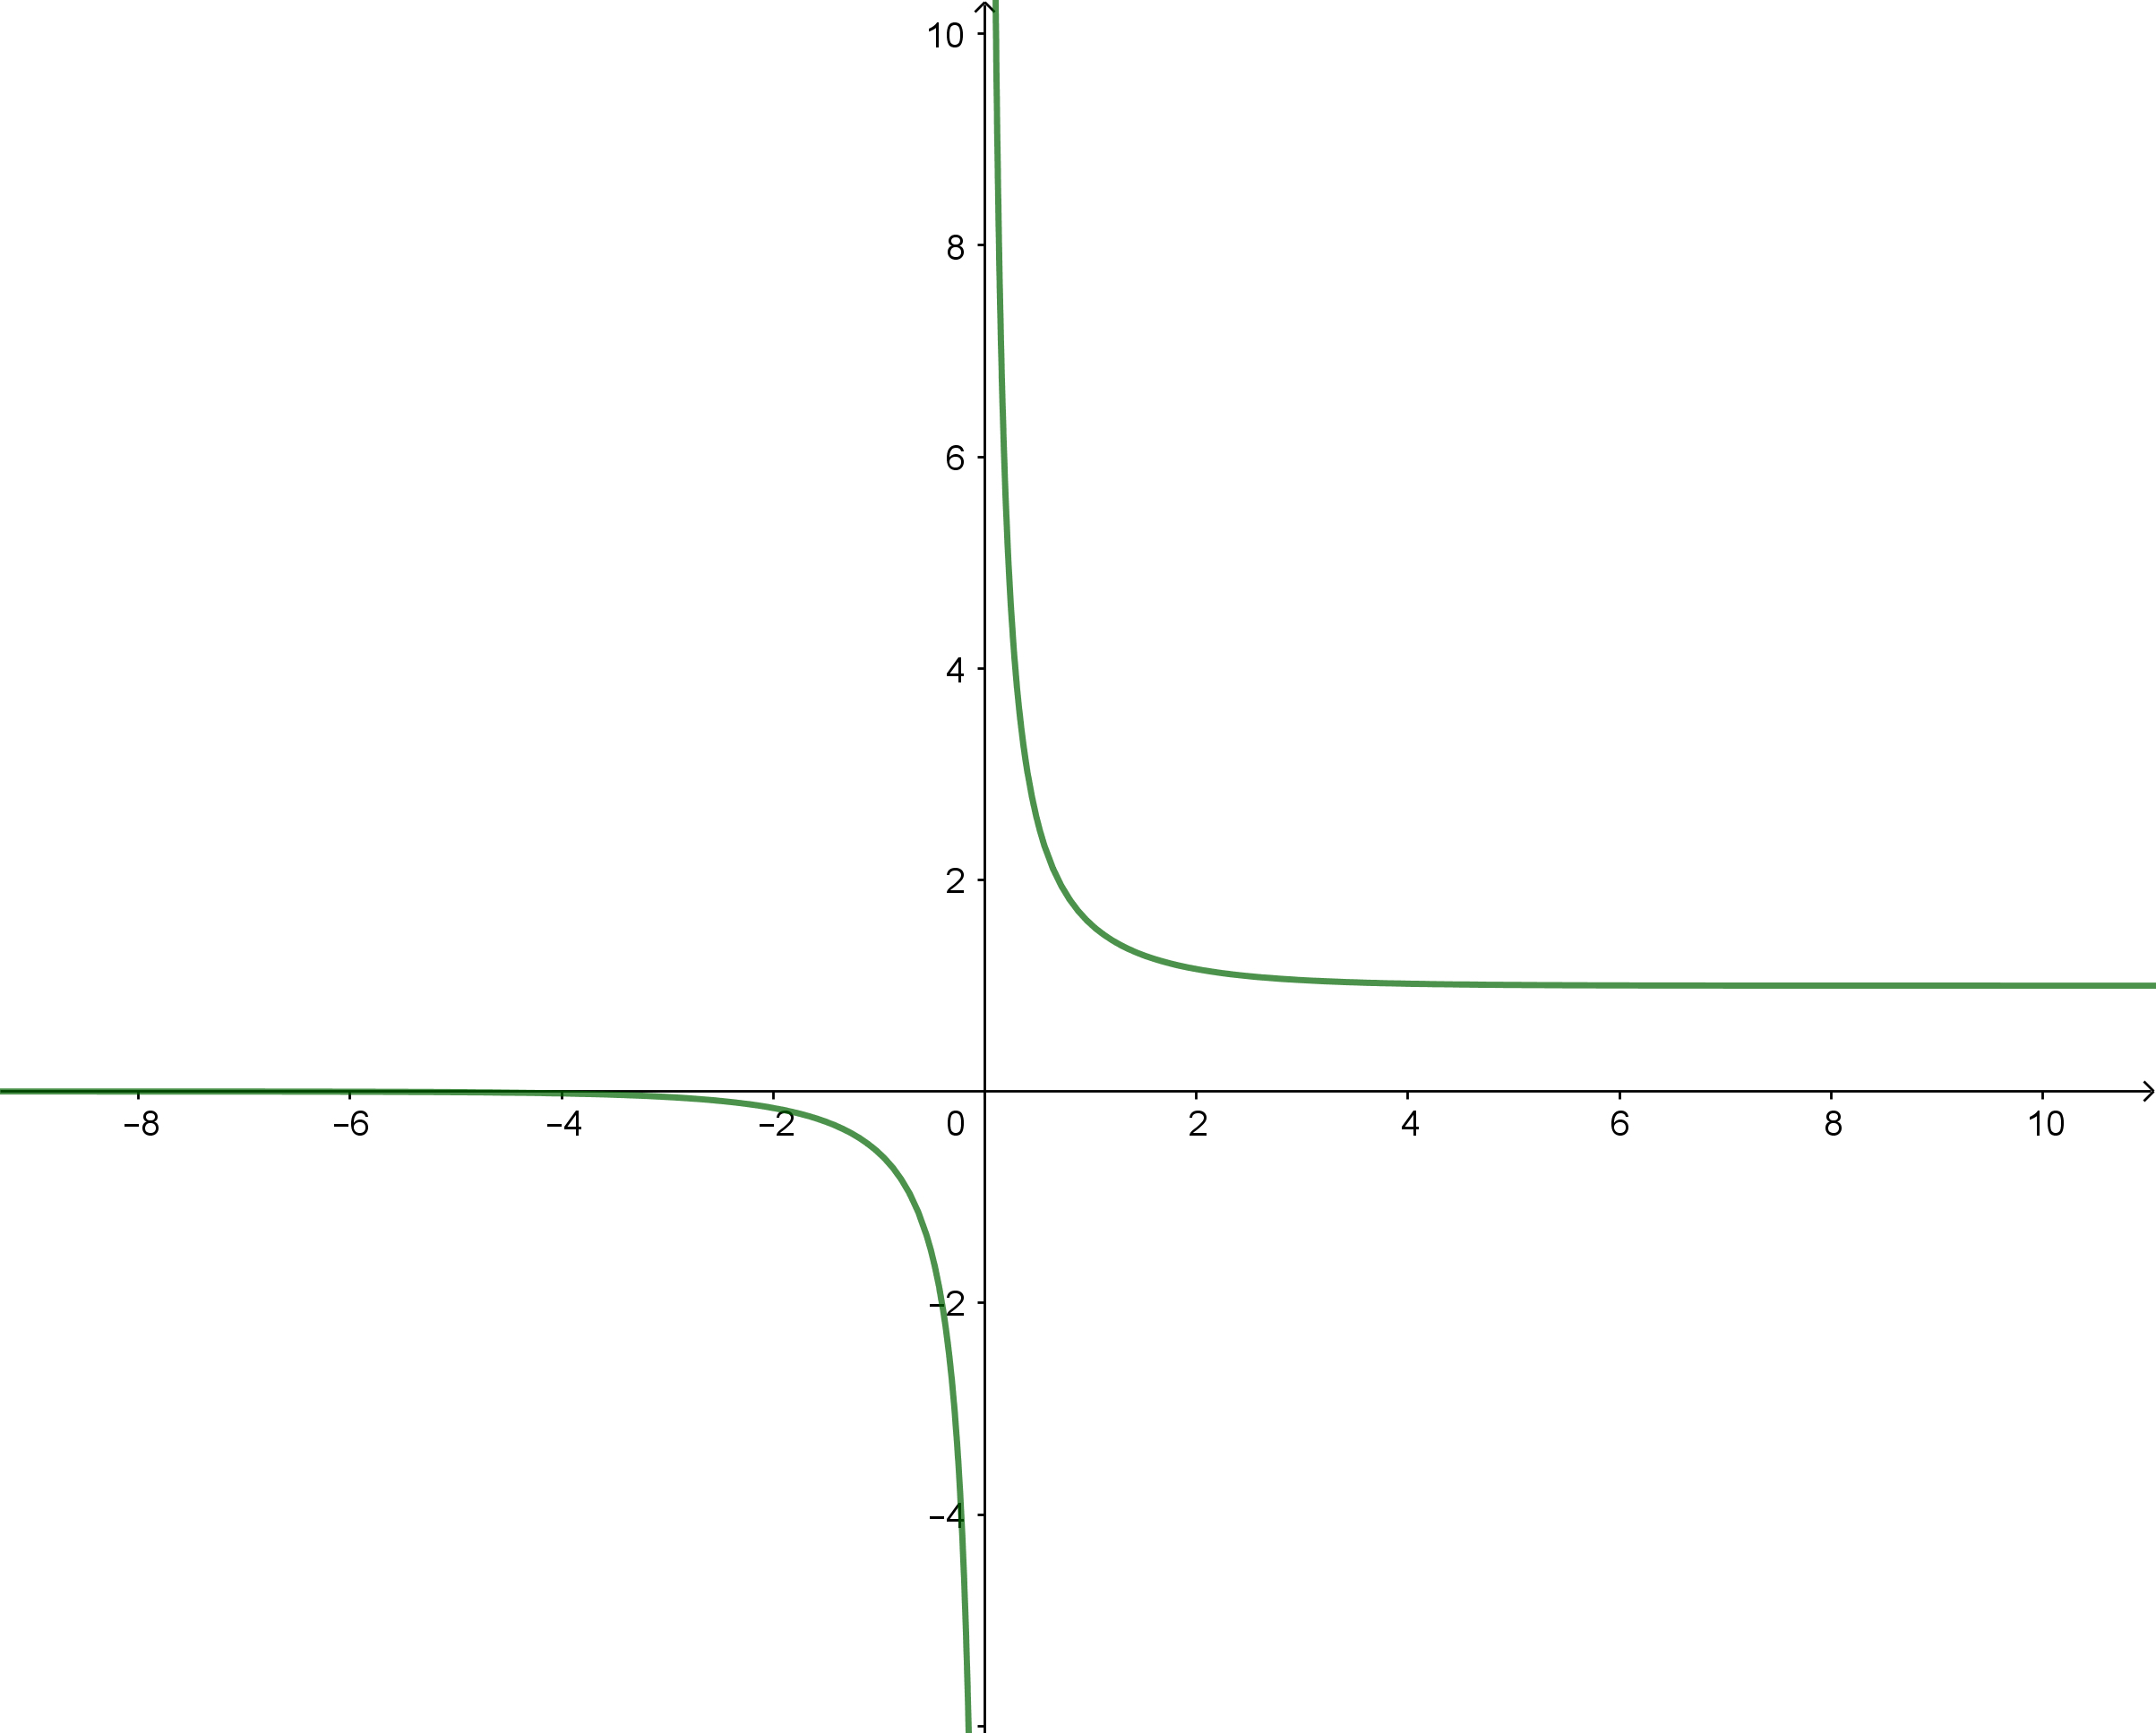
\includegraphics[width=\textwidth]{graphs/sigmoid}
				        \caption{$\sigma$}
				    \end{subfigure}
				    \begin{subfigure}[b]{0.3\textwidth}
				        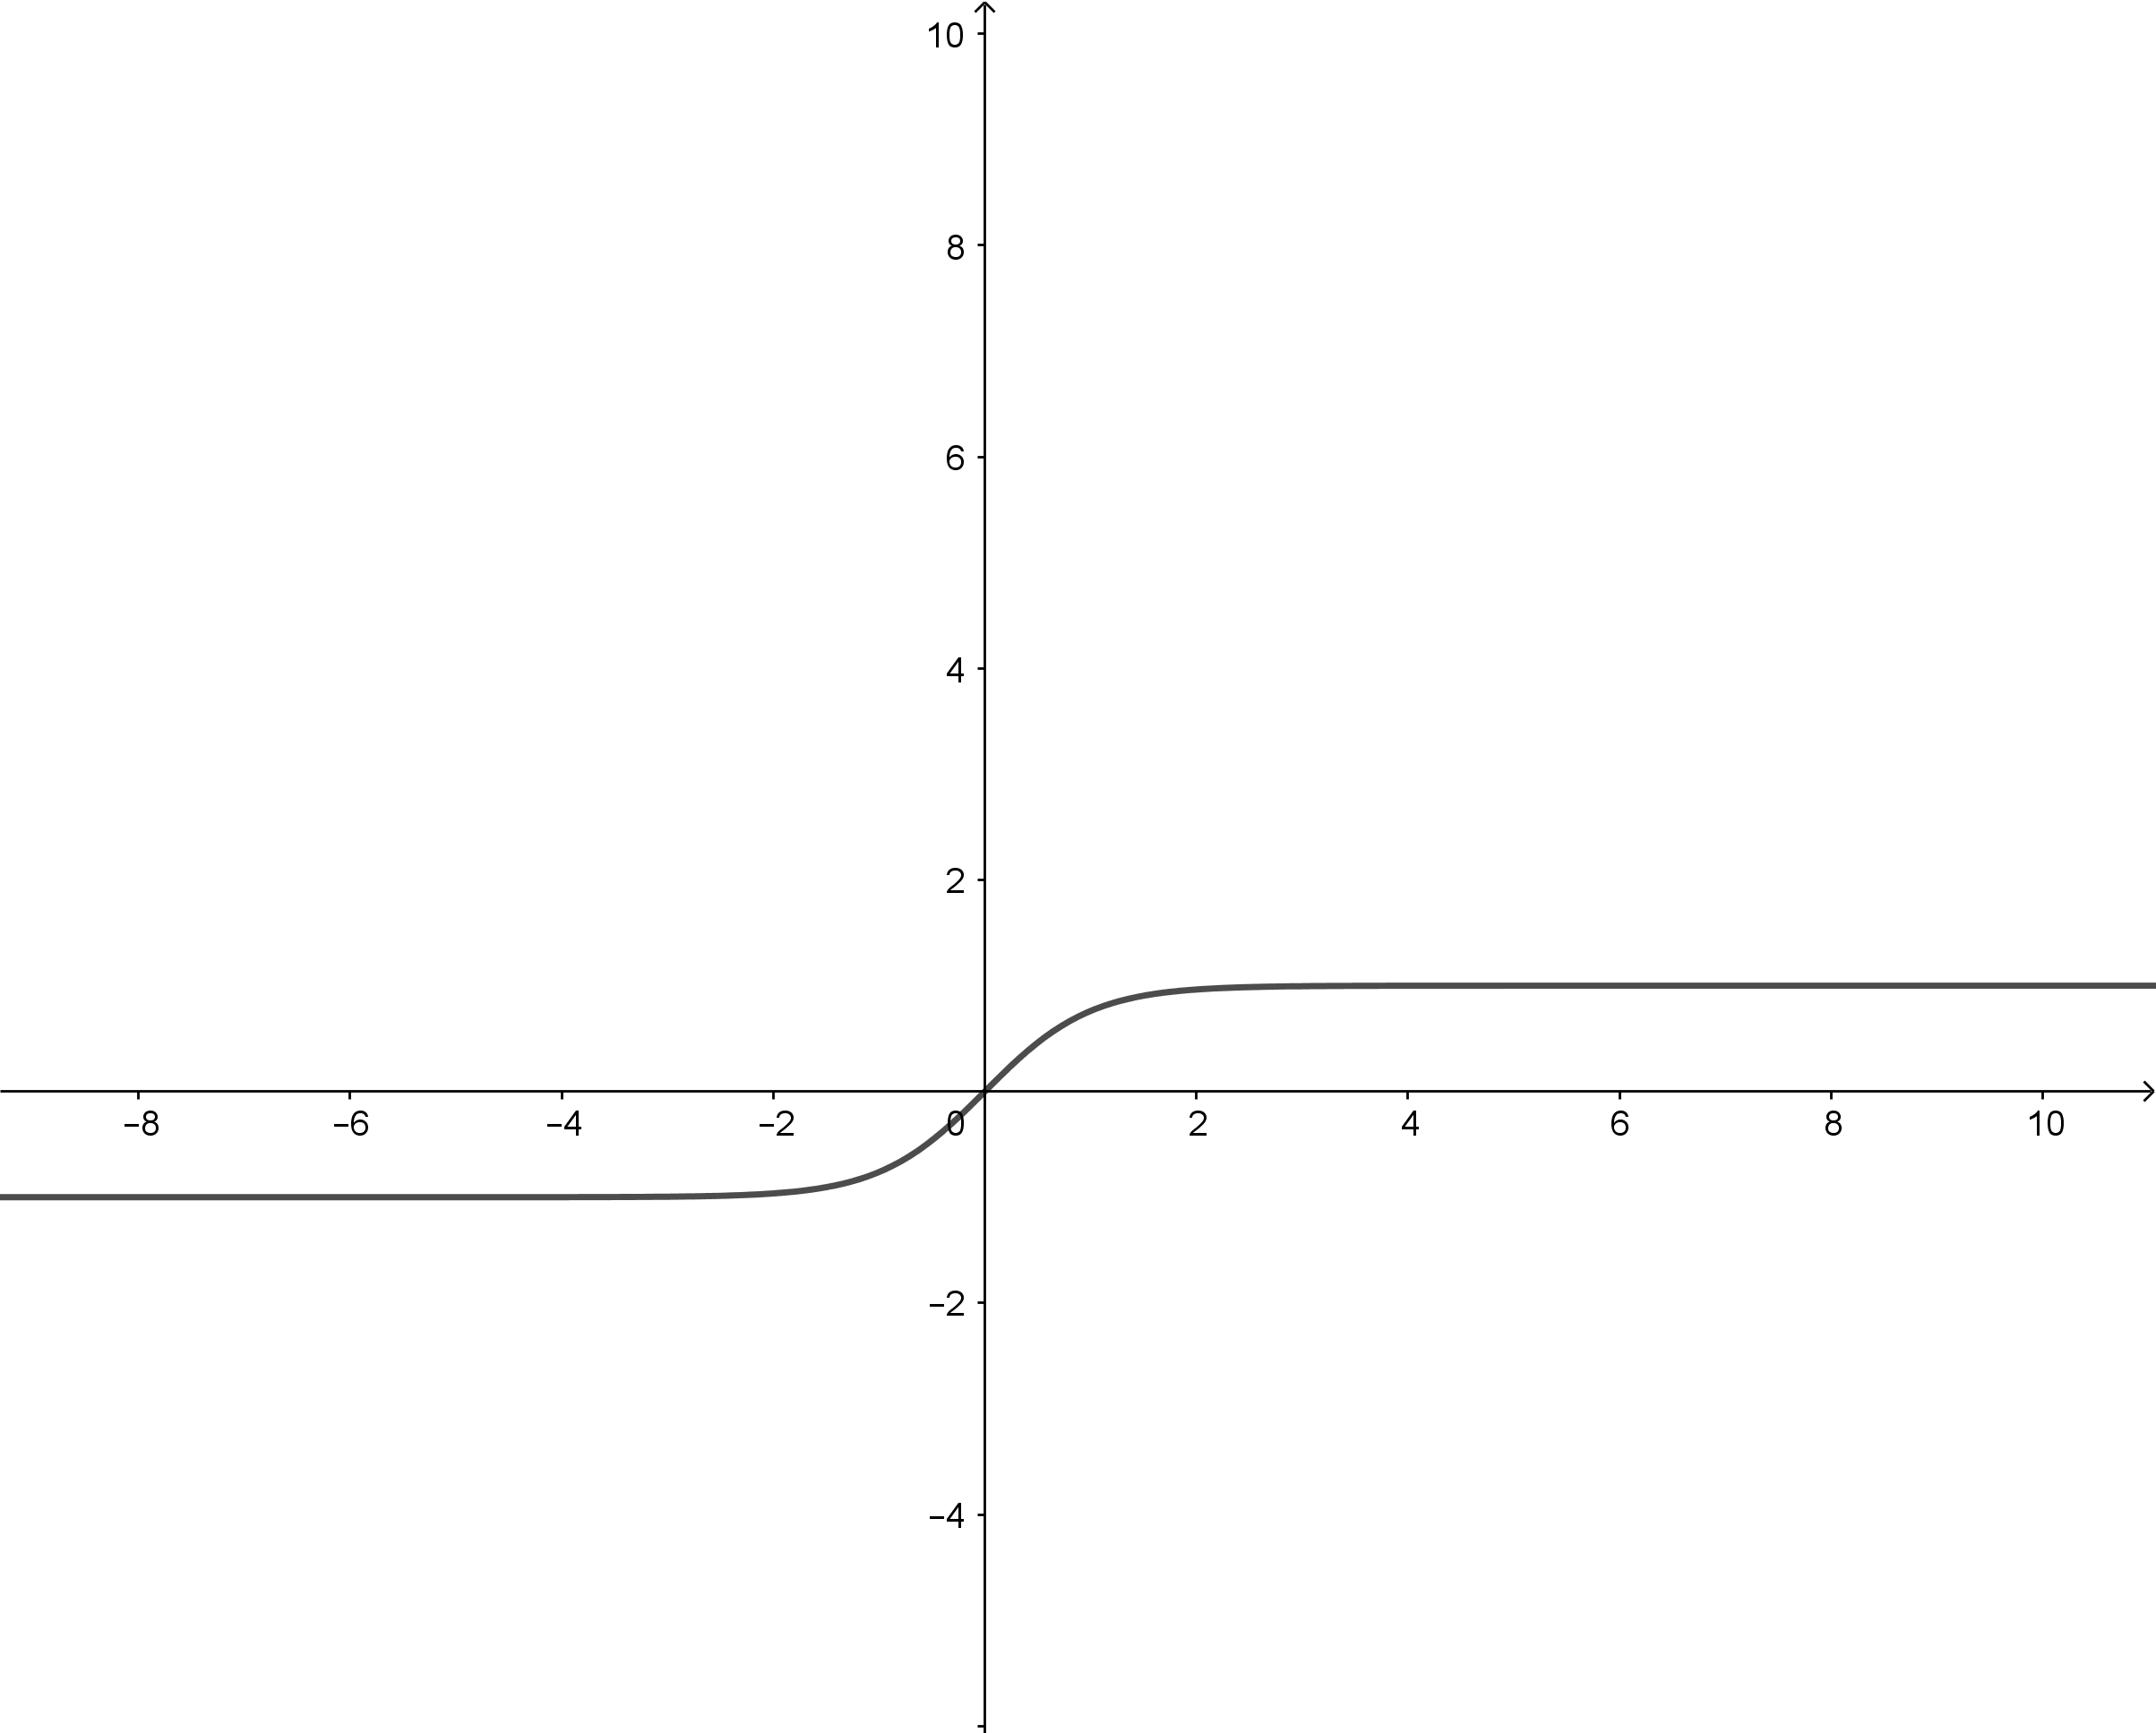
\includegraphics[width=\textwidth]{graphs/tanh}
				        \caption{Hyperbolický tangens}
				    \end{subfigure}
				    \begin{subfigure}[b]{0.3\textwidth}
				        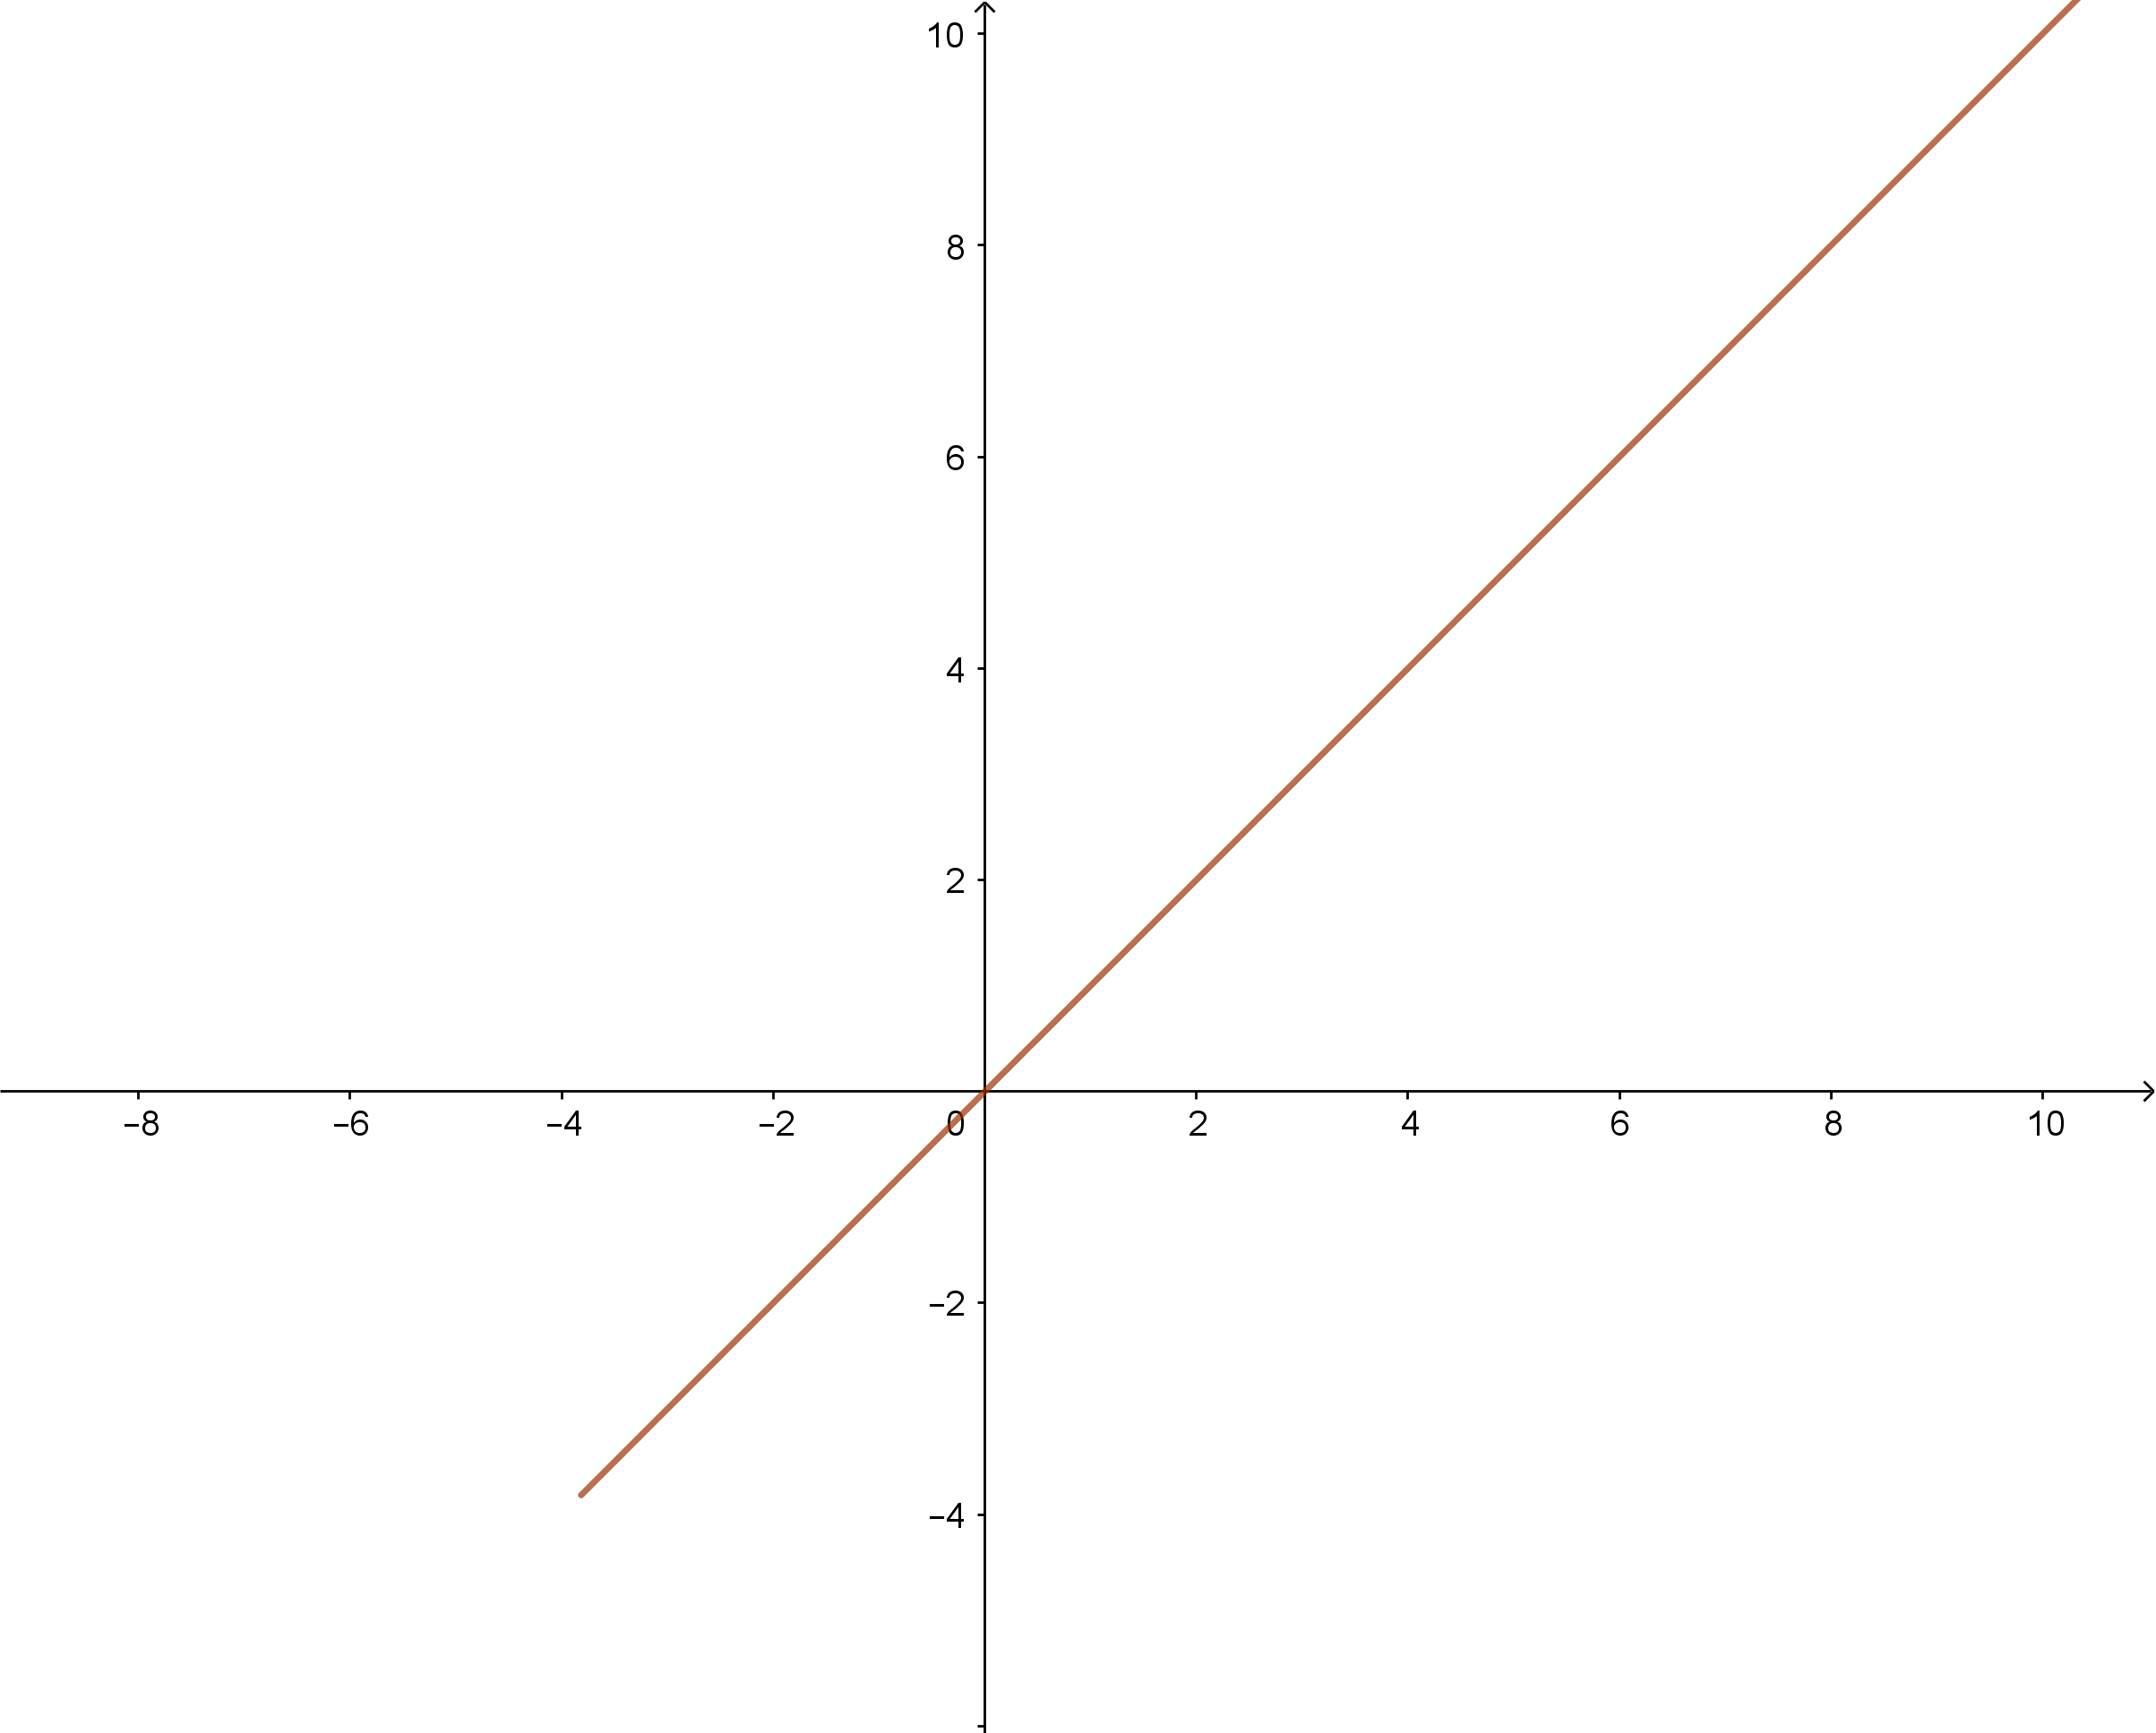
\includegraphics[width=\textwidth]{graphs/identity}
				        \caption{Identita}
				    \end{subfigure}
				    \begin{subfigure}[b]{0.3\textwidth}
				        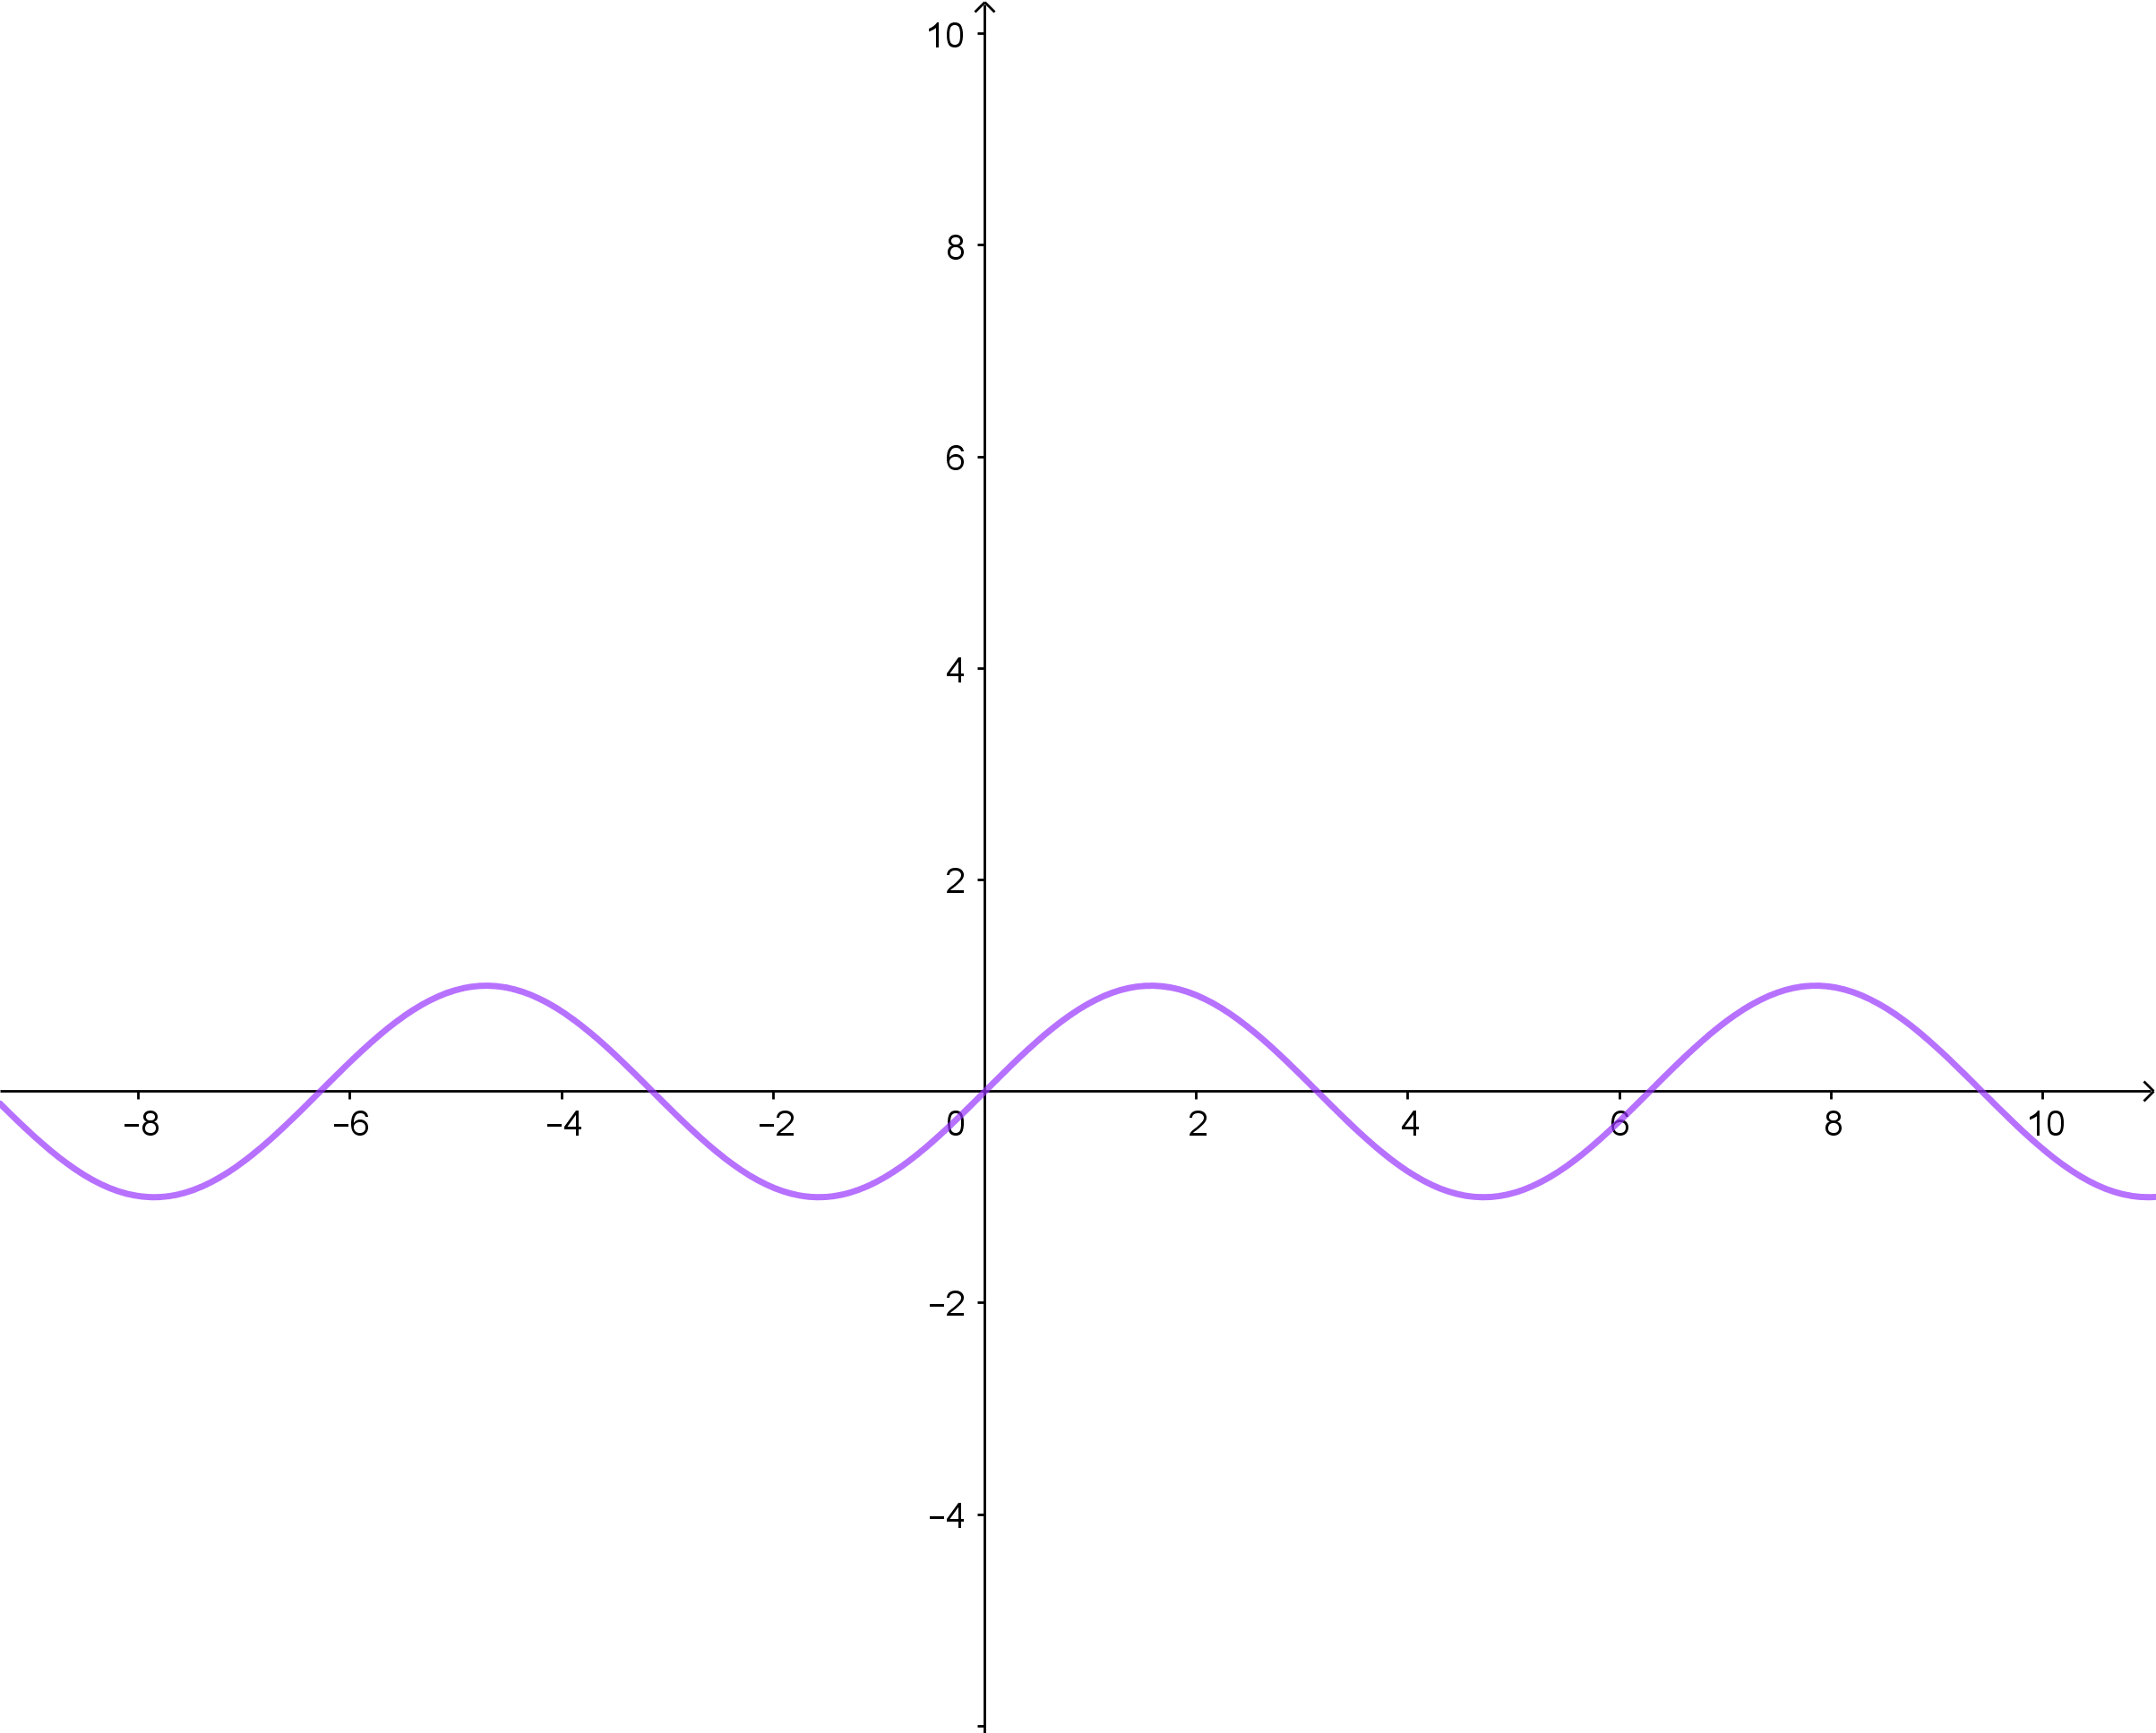
\includegraphics[width=\textwidth]{graphs/sin}
				        \caption{Sinus}
				    \end{subfigure}
				    \begin{subfigure}[b]{0.3\textwidth}
				        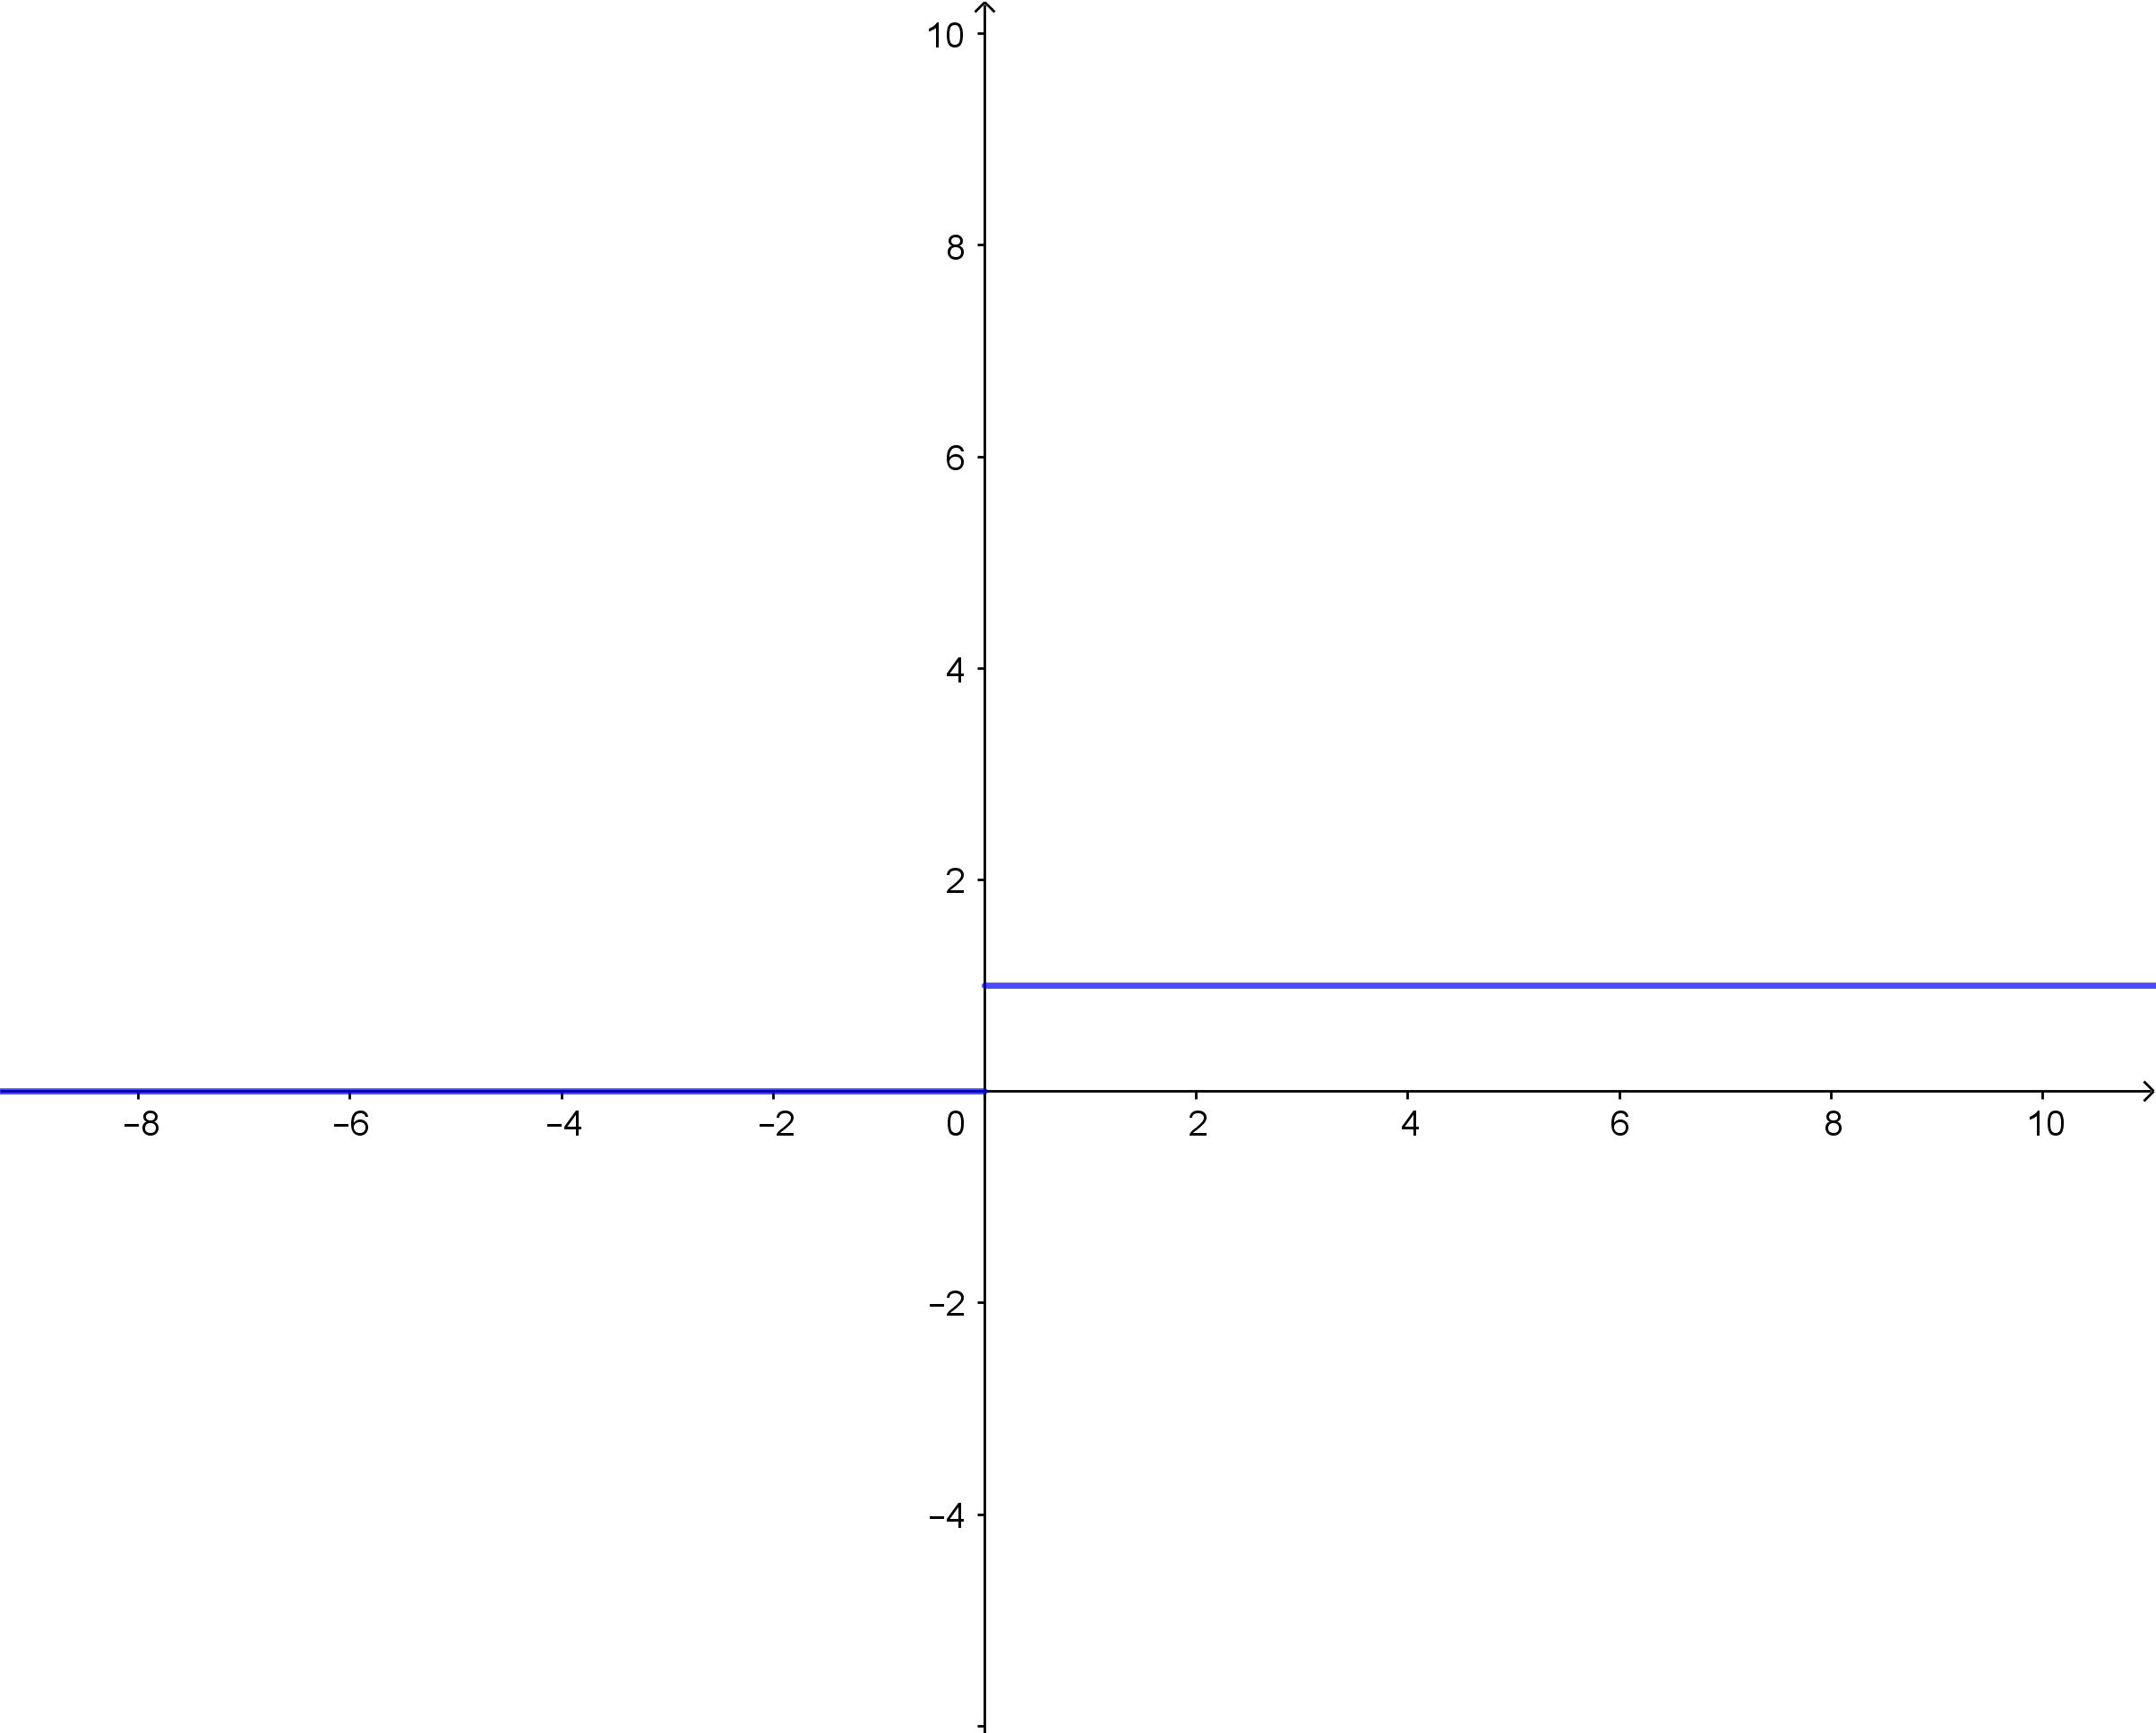
\includegraphics[width=\textwidth]{graphs/binaryStep}
				        \caption{Binární krok}
				    \end{subfigure}
				    \begin{subfigure}[b]{0.3\textwidth}
				        
\includegraphics[width=\textwidth]{graphs/rectifiedLinearUnit}
				        \caption{Rectified linear unit}
				    \end{subfigure}
				    \begin{subfigure}[b]{0.3\textwidth}
				        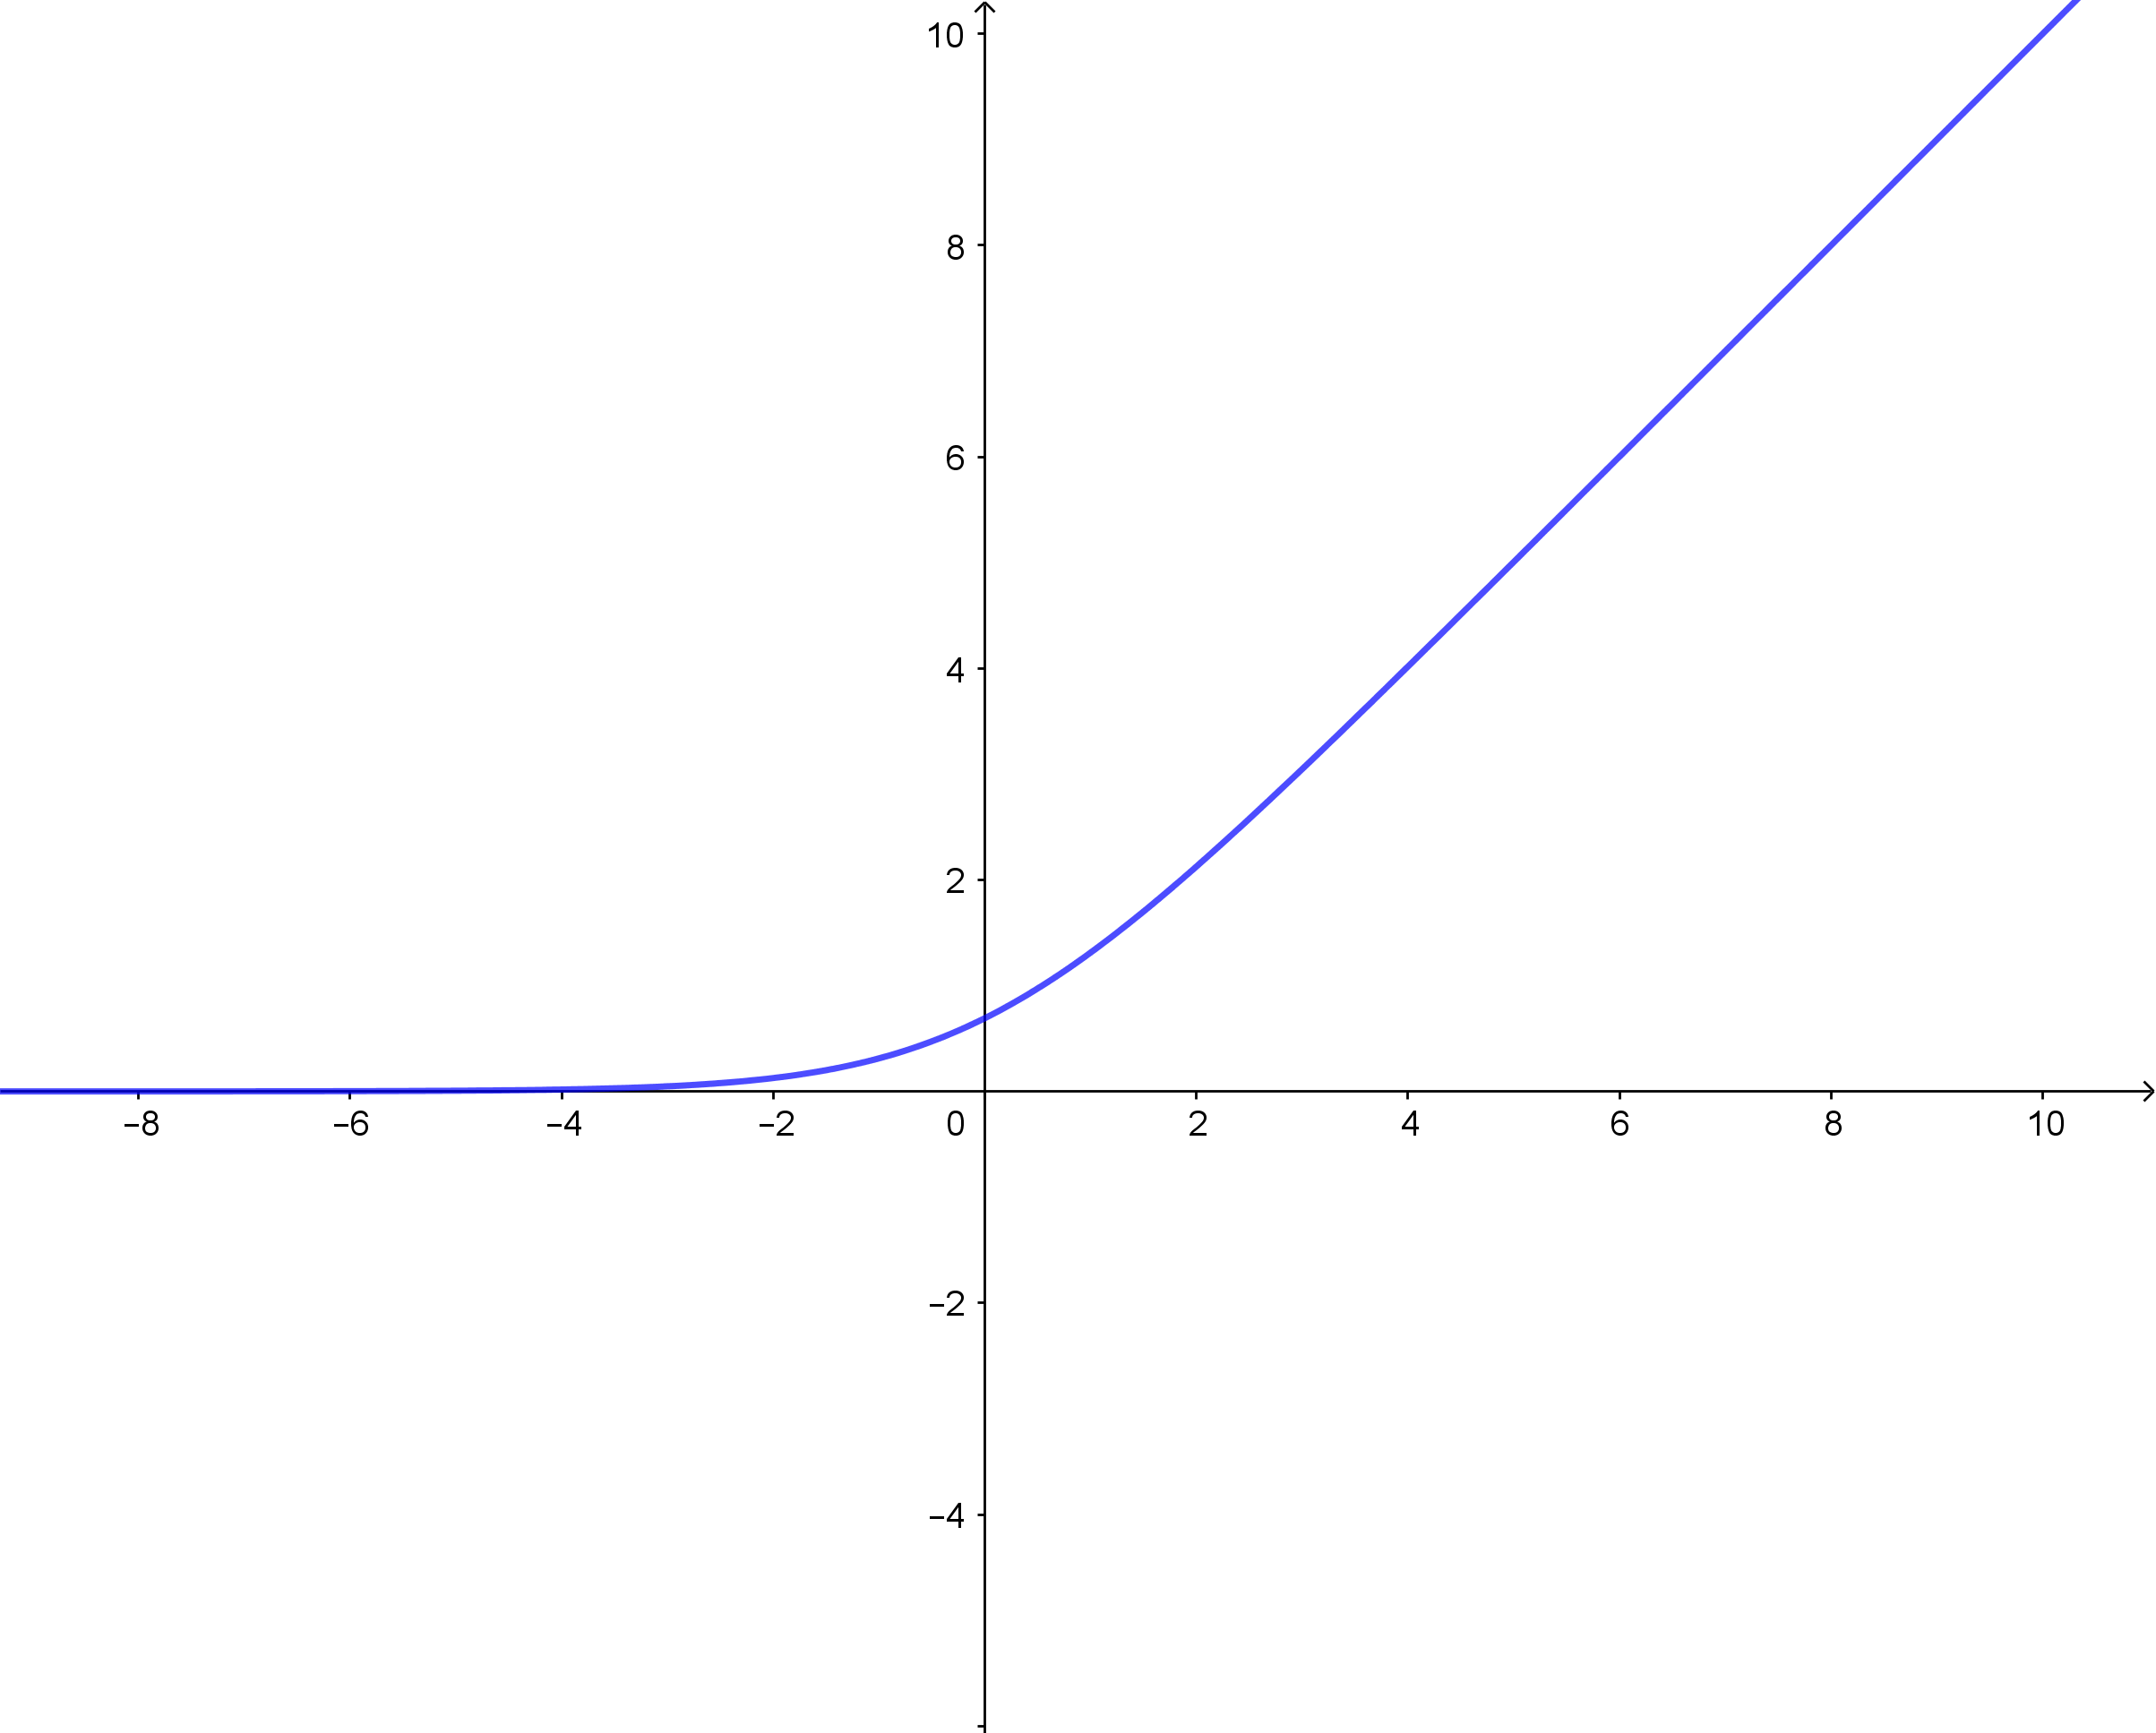
\includegraphics[width=\textwidth]{graphs/softPlus}
				        \caption{Soft plus}
				    \end{subfigure}
				    \begin{subfigure}[b]{0.3\textwidth}
				        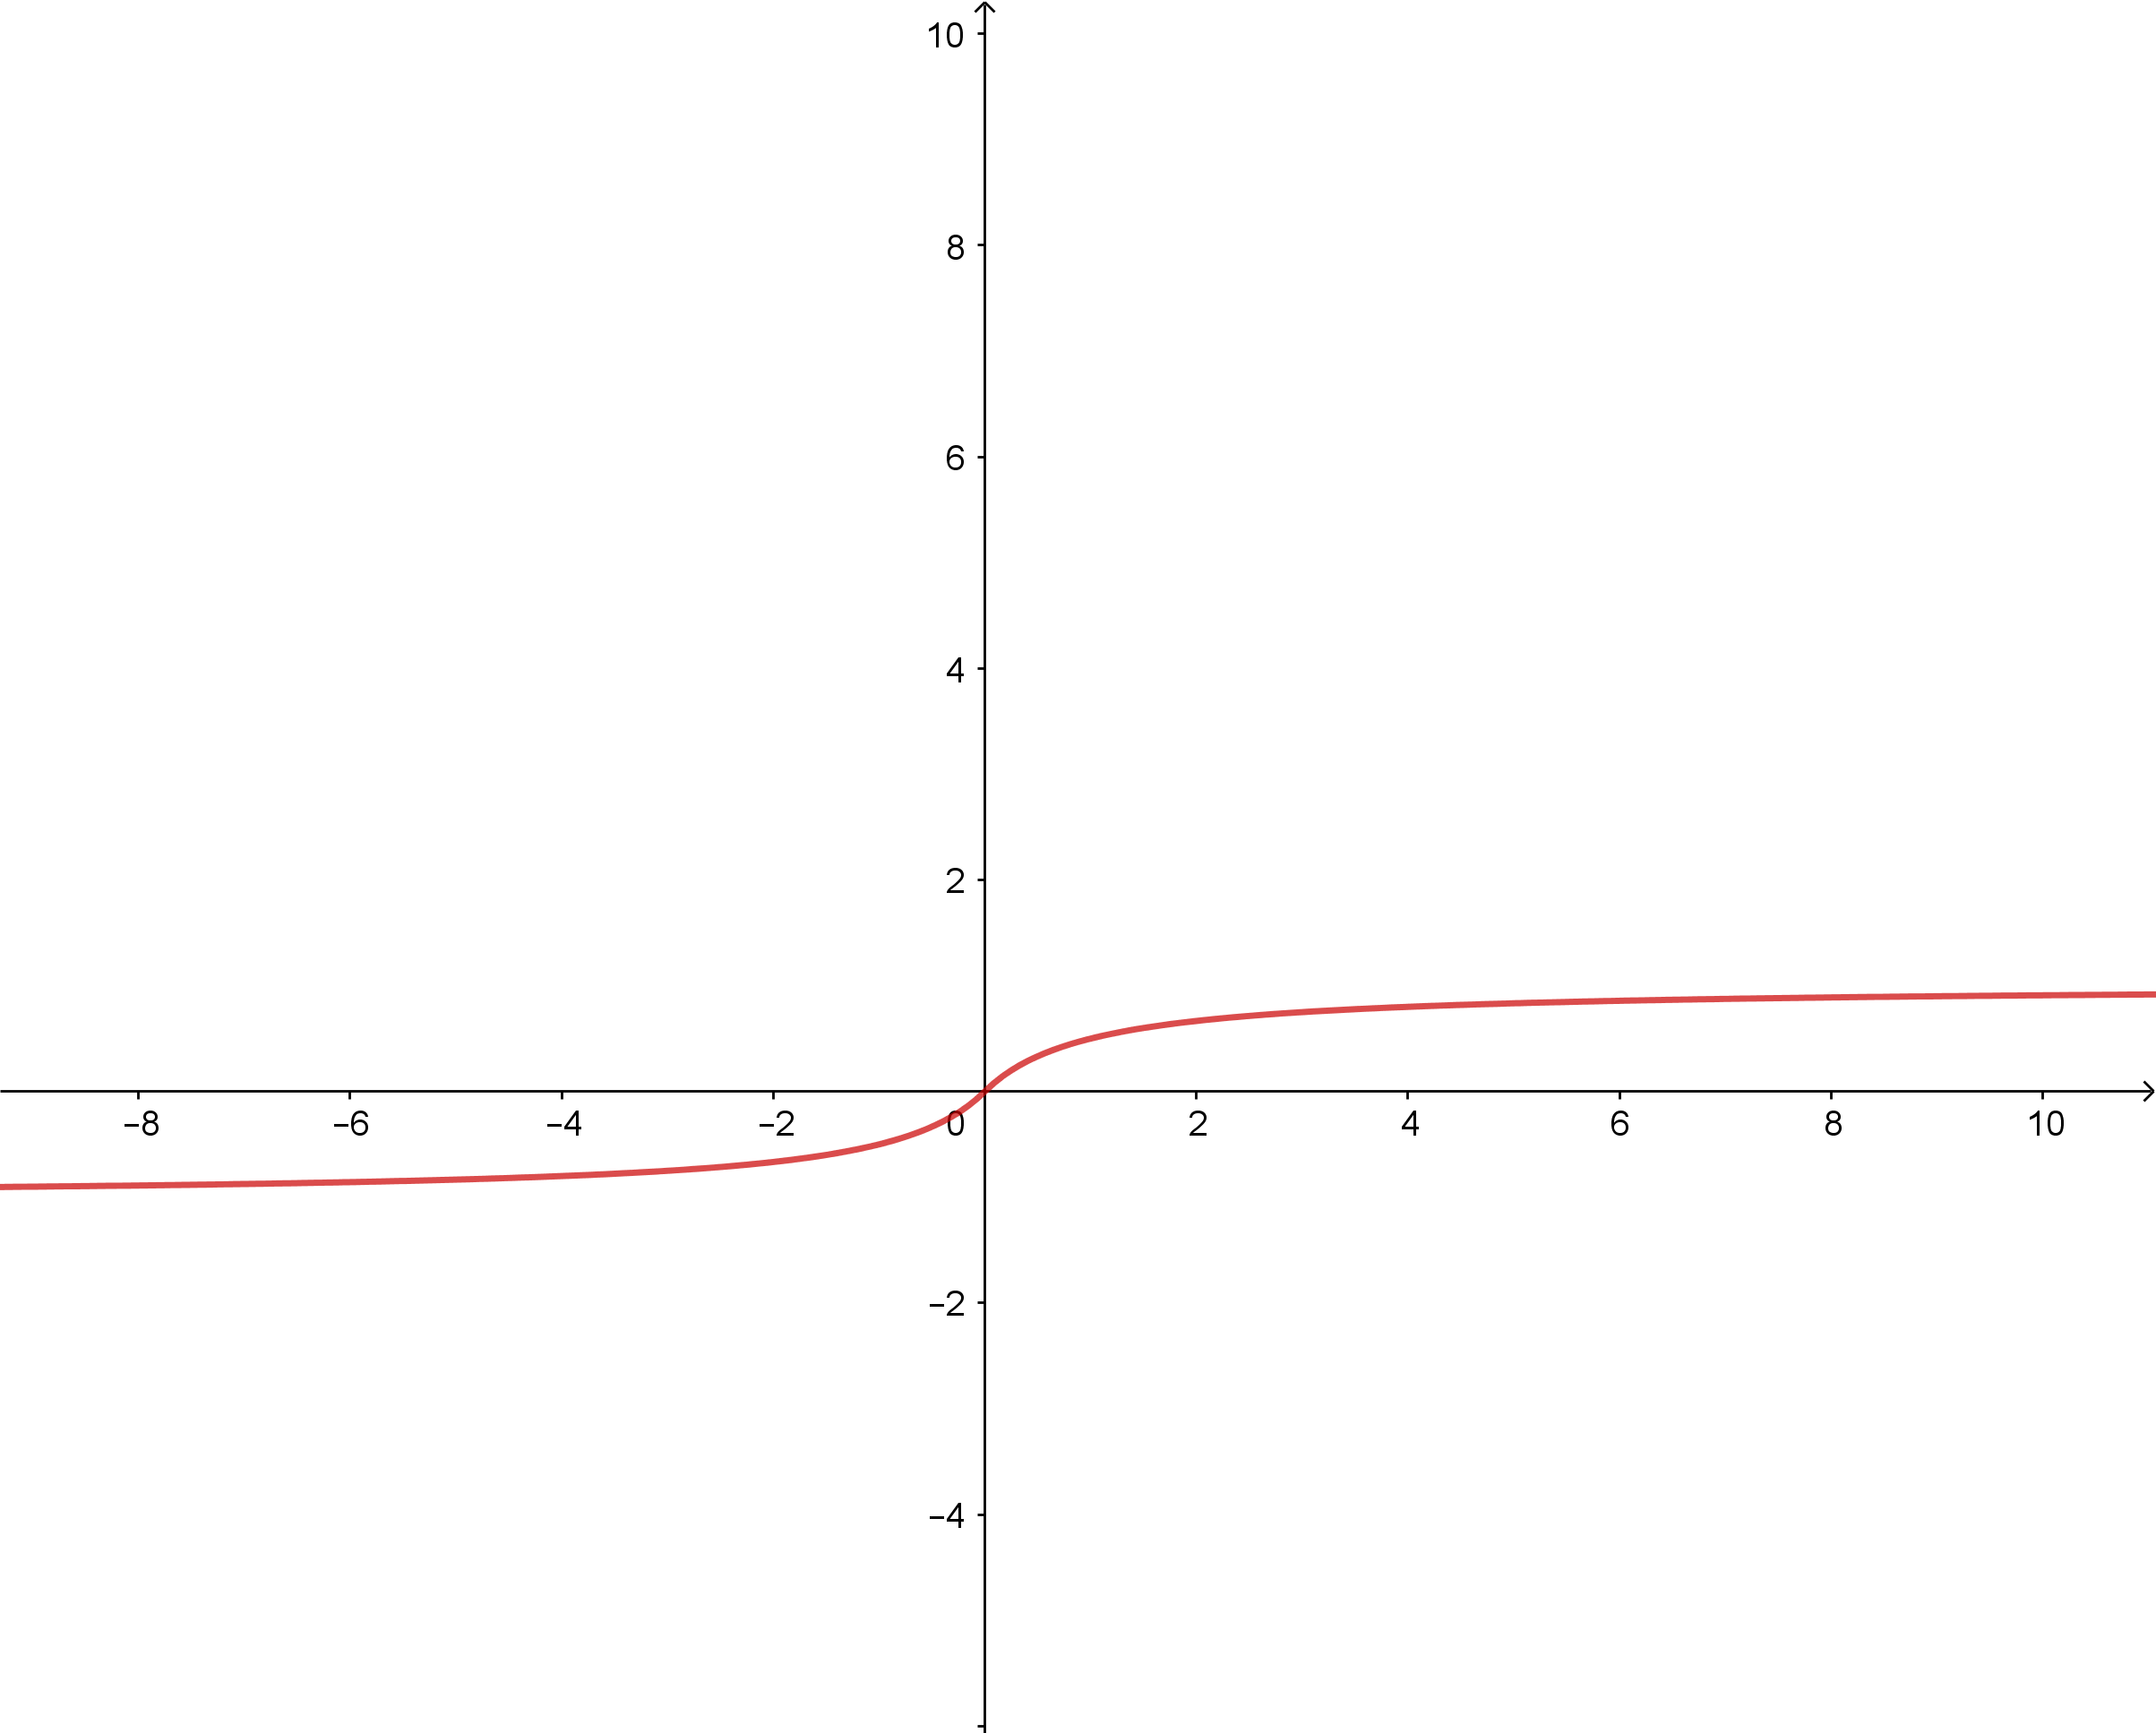
\includegraphics[width=\textwidth]{graphs/softSign}
				        \caption{Soft signum}
				    \end{subfigure}
				    \begin{subfigure}[b]{0.3\textwidth}
				        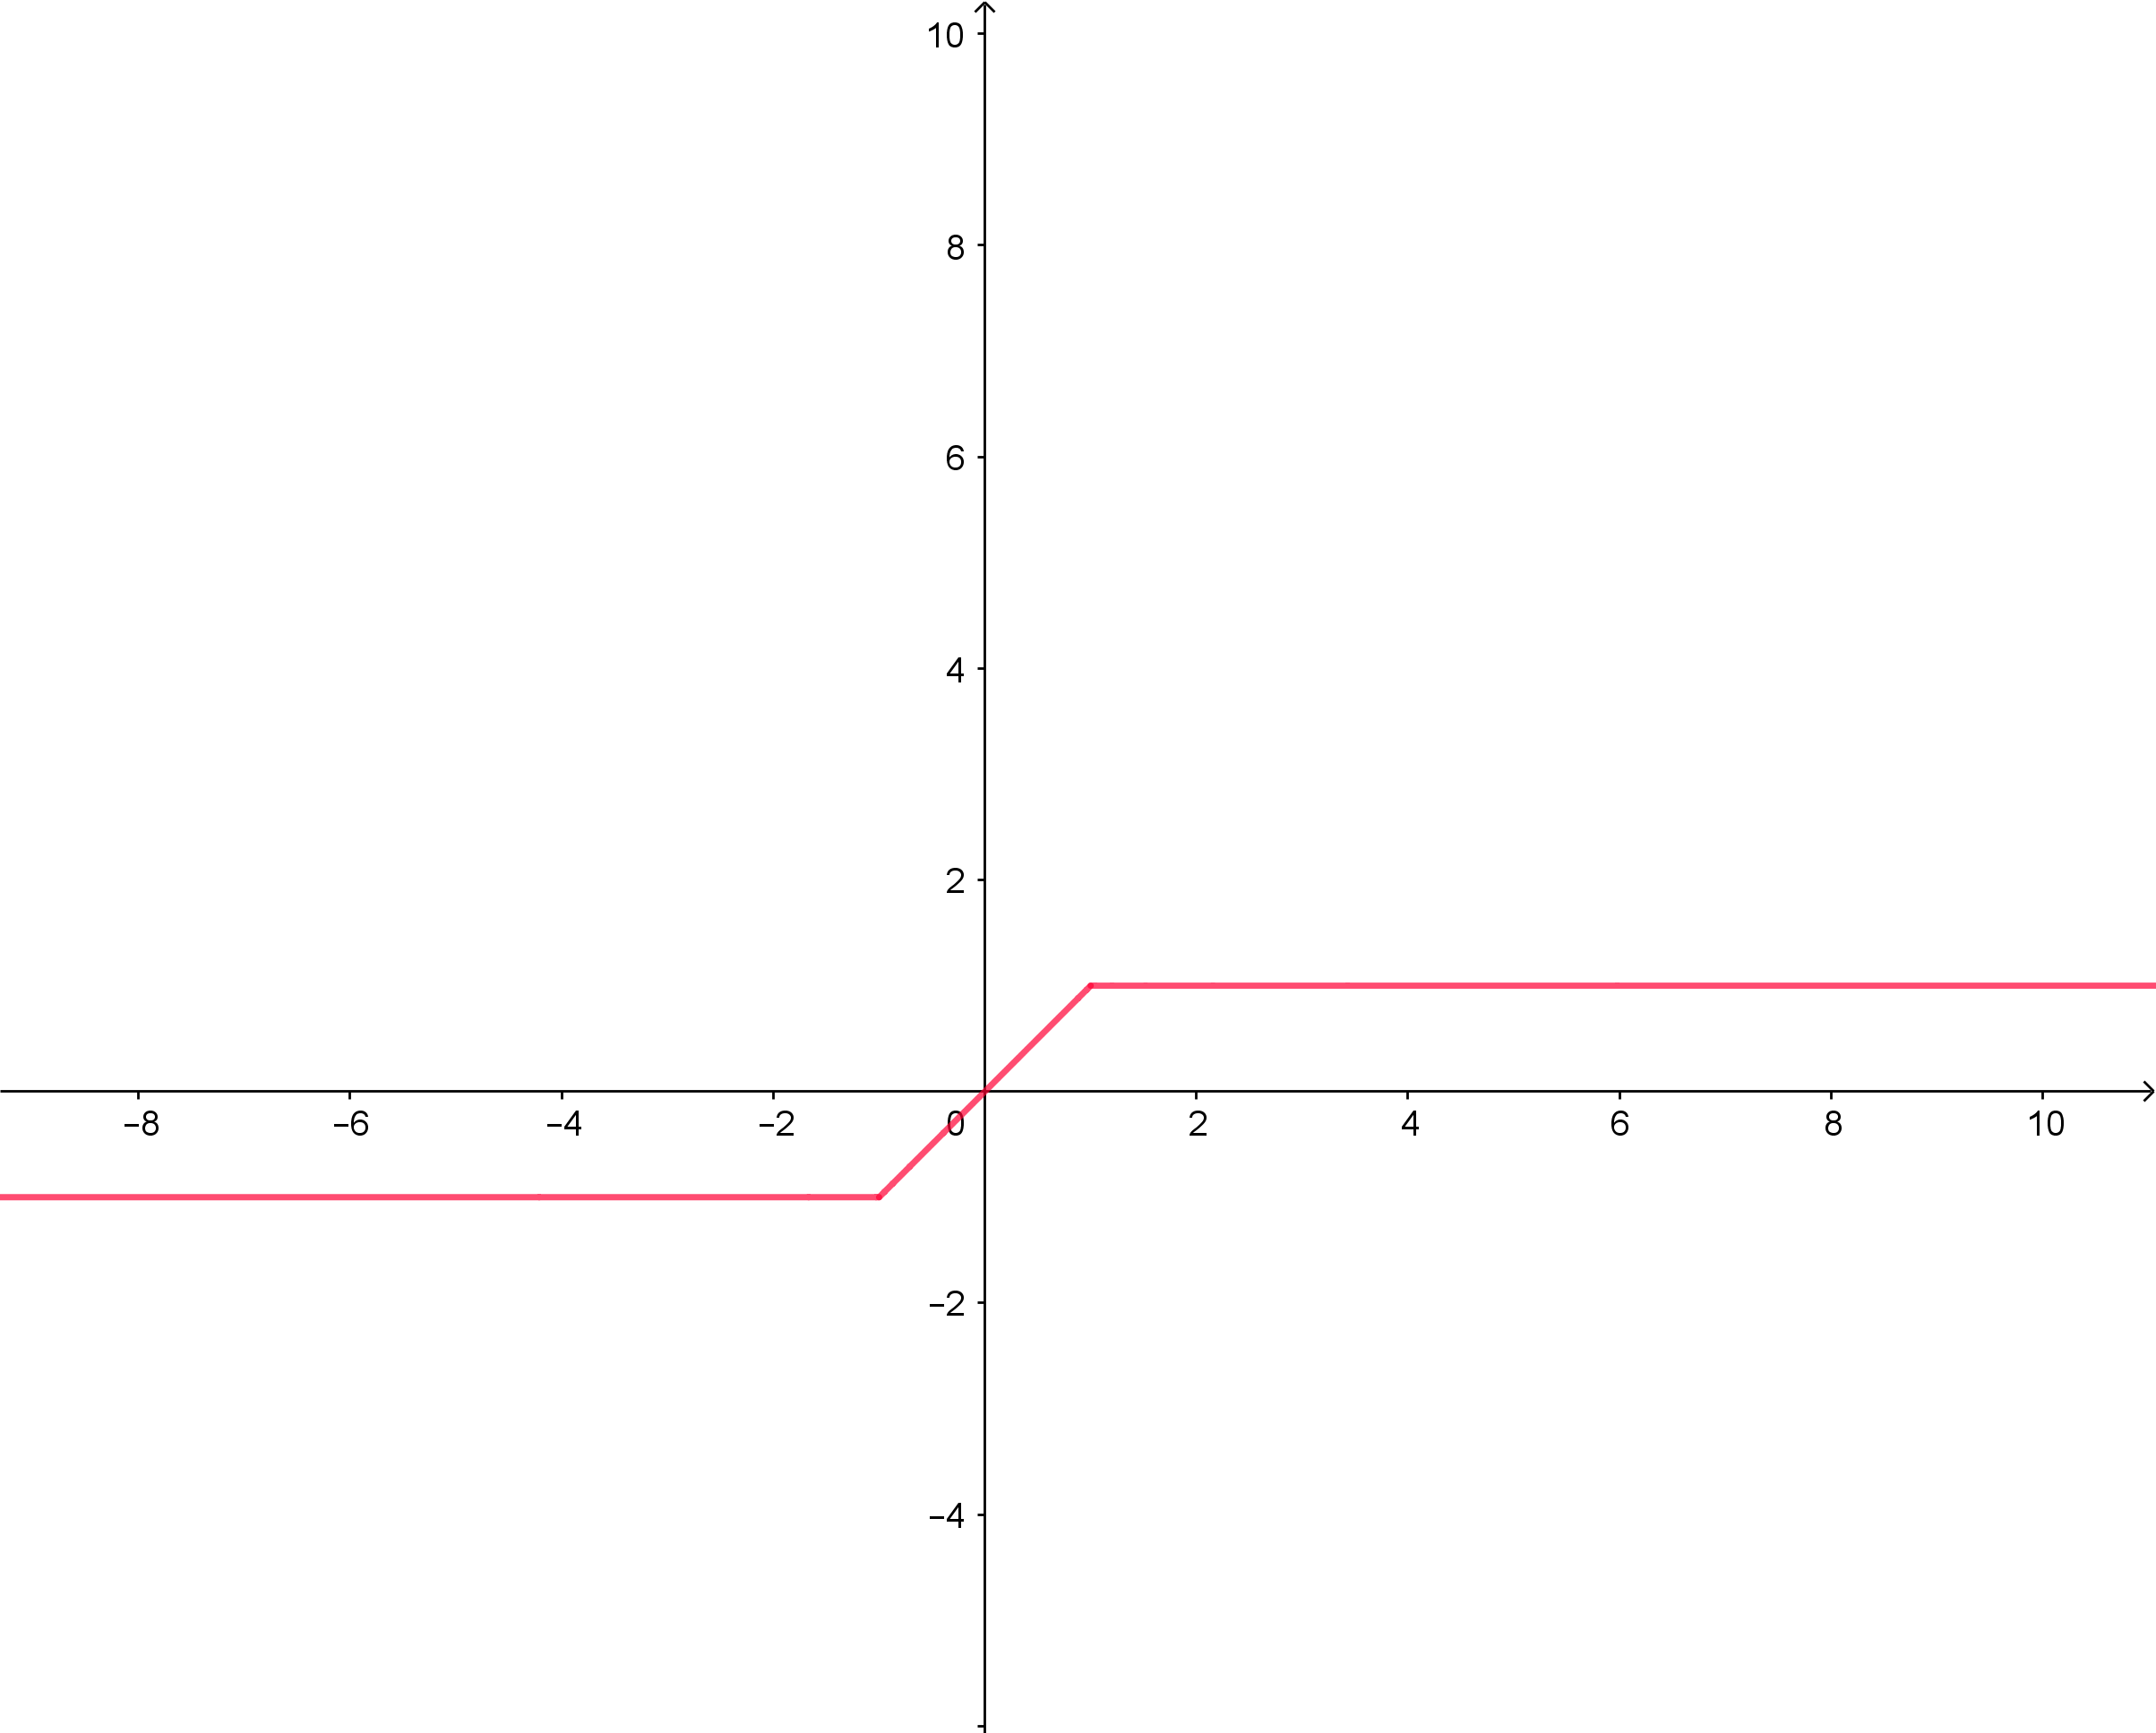
\includegraphics[width=\textwidth]{graphs/hardHyperbolicFunction}
				        \caption{Hard hyperbolic function}
				    \end{subfigure}
				    \begin{subfigure}[b]{0.3\textwidth}
				        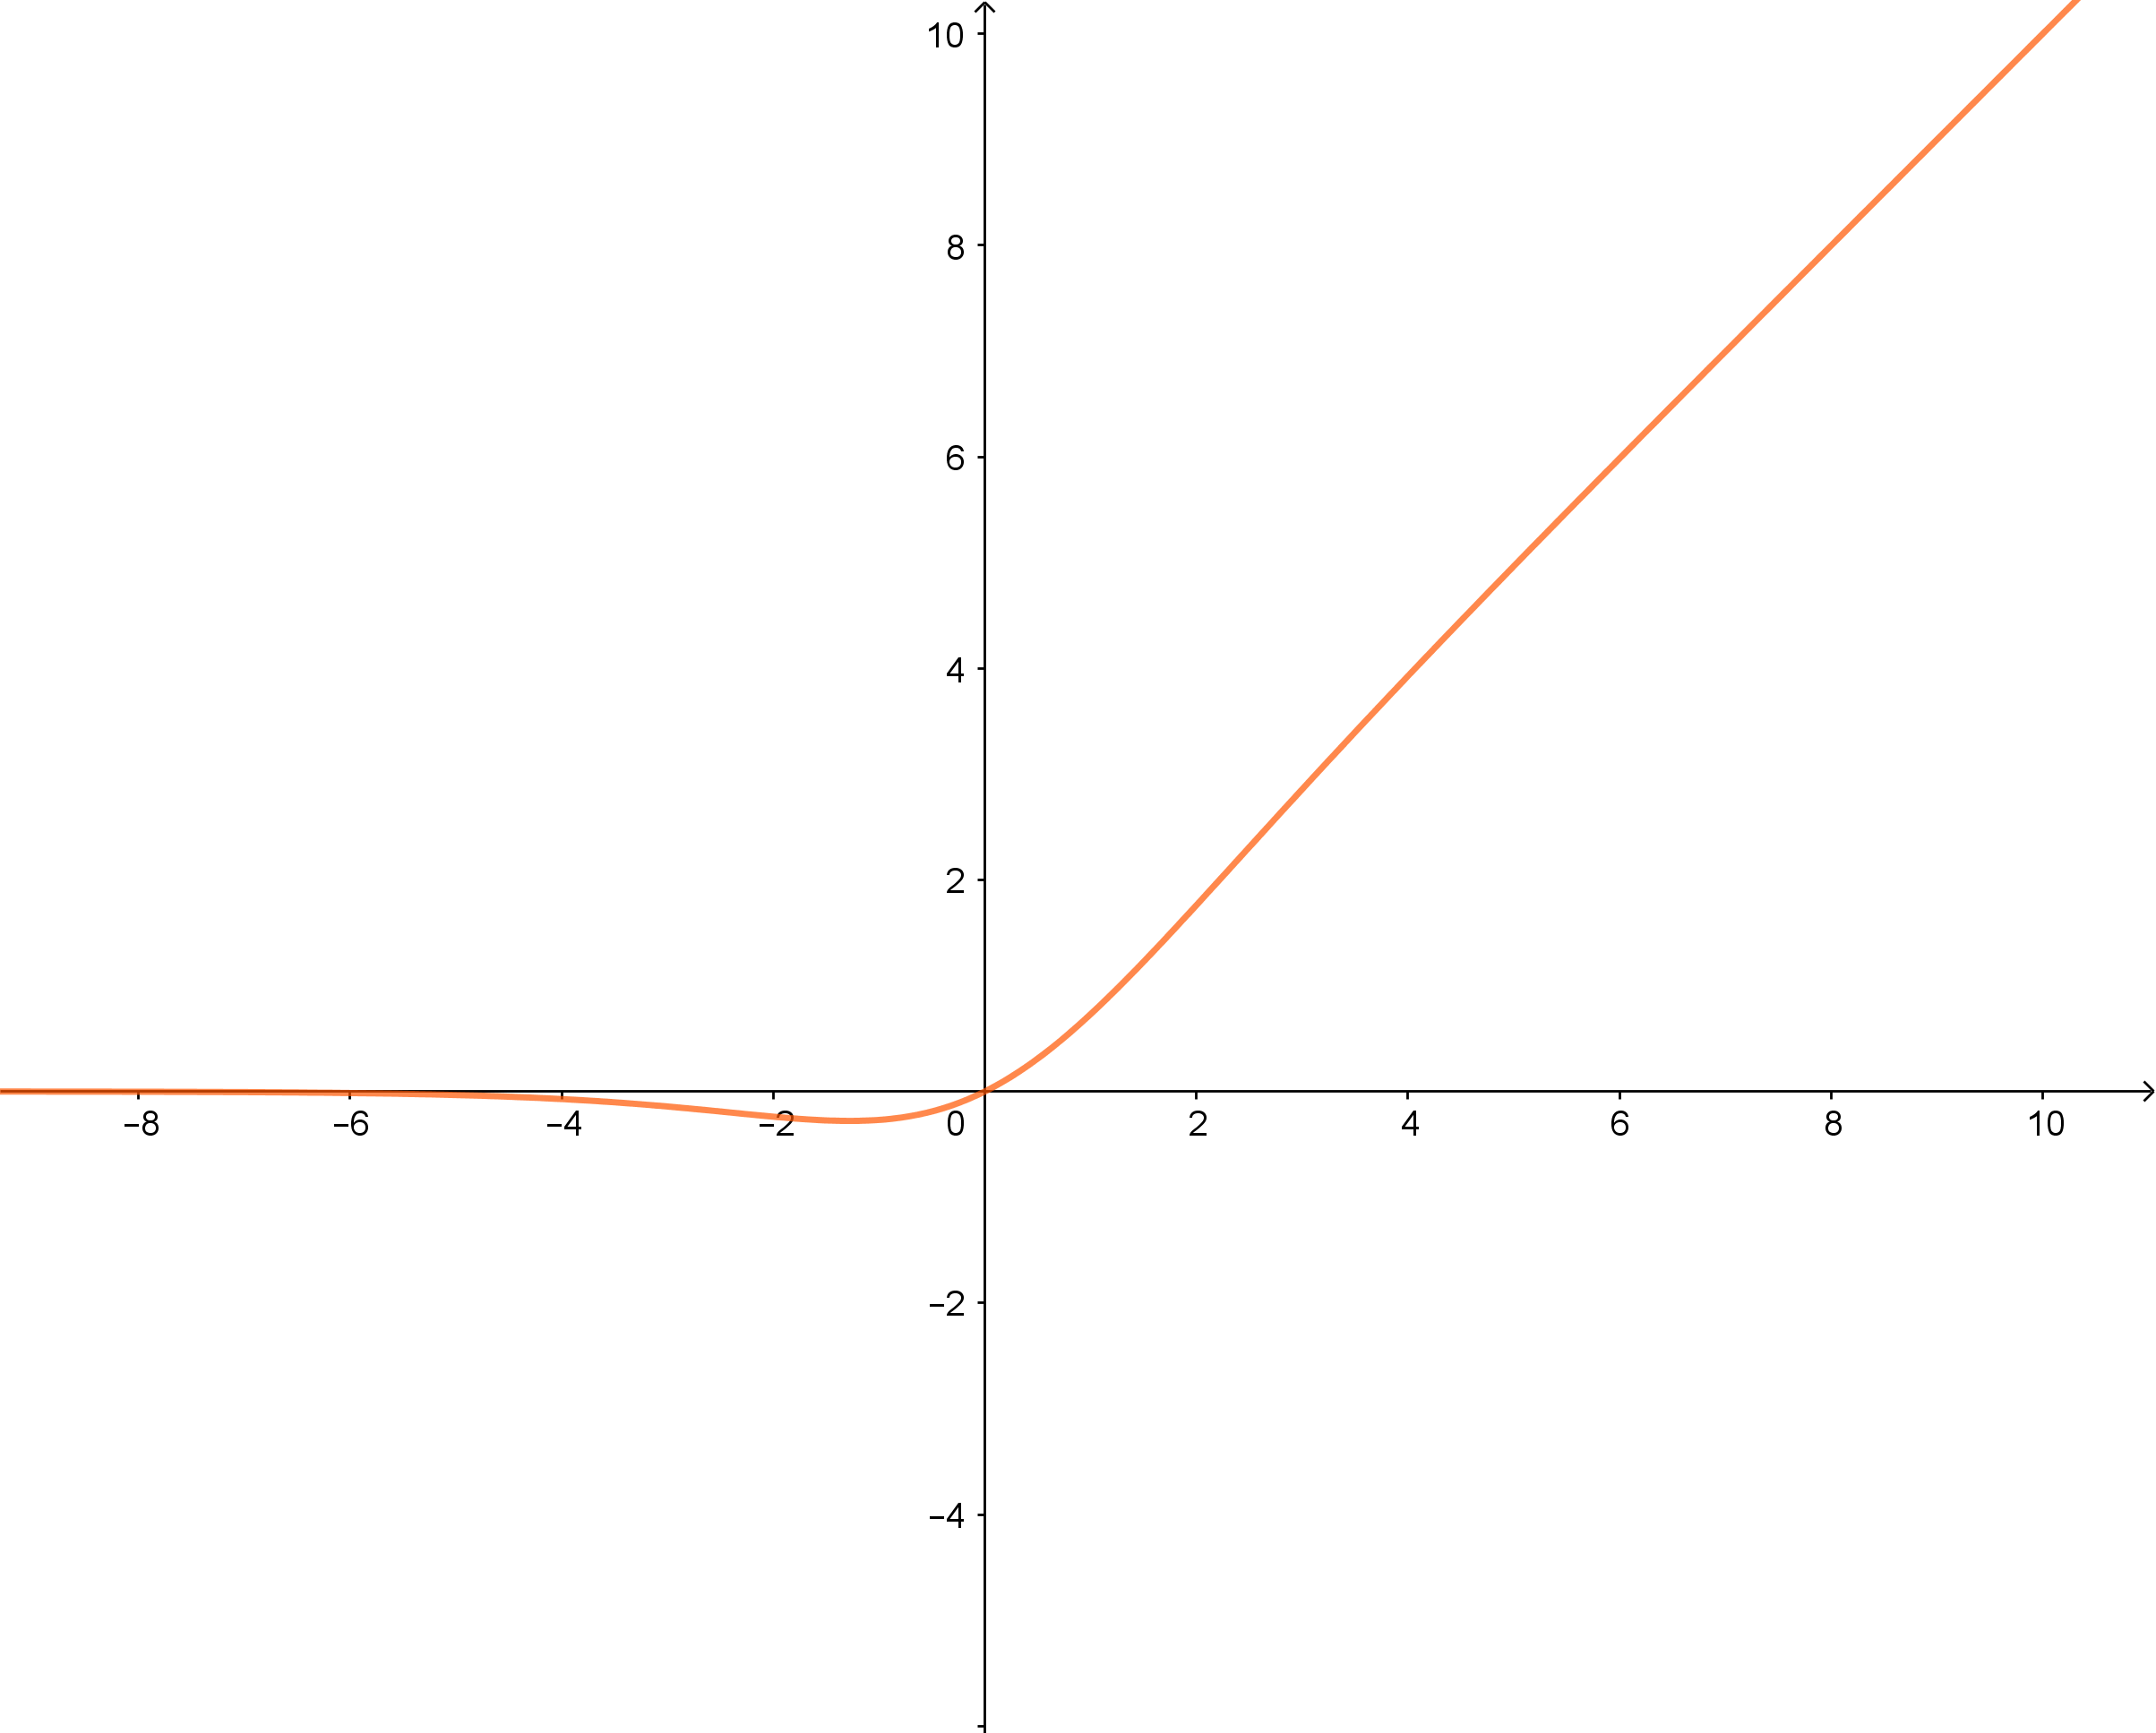
\includegraphics[width=\textwidth]{graphs/swift}
				        \caption{Swift}
				    \end{subfigure}
				    \caption{Aktivační funkce (vyrobeny v programu Geogebra)}
				\end{figure}
						
				\end{itemize}
				
			
		
	\part{Praktická část}
	
		\chapter{Struktura knihovny}
			Knihovna je rozdělena do dvou částí:
			\begin{itemize}
				\item První, a ta hlavní, je core (česky jádro), které obsahuje definice neuronových sítí (tj. konvoluční neuronovou síť, obyčejnou neuronovou síť, asociativní paměť) a definice pro ně potřebné (například aktivační funkce).
				\item Druhá je mnistDatabase, která se stará o učení neuronových sítí na datových databázích.
			\end{itemize}
			
			\section{core}
			
				\subsection{ActivationFunctions}
					Enumerate (česky výčet) funkcí, jež se používají jako aktivační funkce v neuronech. Funkce lze zavolat s parametrem typu \verb!Double!, což nám dá hodnotu funkce v tomto bodě, popřípadě lze obdobně zavolat jejich 2 metody \verb!xD! a \verb!yD! udávající v pořadí hodnotu derivace v bodě x a v bodě, kde je funkční hodnota rovna parametru.\footnote{Druhá hodnota se používá, jelikož při zpětné propagaci máme k dispozici i funkční hodnotu, a derivace se u těchto funkcí často jednodušeji spočítá právě z této hodnoty.}
					
					Některé jsou označeny jako překonané (anglicky deprecated), jelikož u funkcí, které nejsou všude hladké, neexistuje všude derivace. Taktéž u funkcí, jež nejsou prosté, nelze vždy určit derivaci podle funkční hodnoty.
					
					Implementovány jsou všechny funkce uvedené v kapitole \ref{s:af}
			
				\subsection{INeuralNetwork}
					Rozhraní (anglicky \gls{interface}), které implementuje základní funkce neuronových sítí, které mají jako vstup i výstup Double (typ pro přesnější desetinné číslo) vektor. Obsahuje funkce:
					\begin{itemize}
						\item \verb!run(vstupní vektor)!, která je koncipována tak, aby ze vstupního vektoru spočítala vektor výstupní (tedy většinou udělala dopřednou propagaci). Jako vstupní vektor lze dát jak \verb!Matrix<Double>! z knihovny \verb!koma!, tak \verb!DoubleArray!, které je převedeno na \verb!Matrix<Double>!, následně se zavolá funkce \verb!run! s tímto typem a výstup se převede zpět na \verb!DoubleArray!.\footnote{\verb!DoubleArray! je použito, protože je to typ Kotlinu samotného, ale jelikož matematika v Neuronových sítích je implementována pomocí \verb!Matrix<Double>!, musí se převést mezi typy.}
						
						Navíc (hlavně kvůli konvolučním neuronovým sítím) může být vstup i dvourozměrný, v tomto případě je pak nutno u \verb!DoubleArray! uvést i šířku řádku.
						\item \verb!train(vstupní vektor, chtěný výstupní vektor)! resp. \verb!train(vstupní vektory, chtěné výstupní vektory)!, která je koncipována tak, aby nejdříve provedla \verb!run(vstupní vektor)!, výsledek porovnala s chtěným a přepočítala váhy v neuronové síti tak, aby se výstup \verb!run(vstupní vektor)! přiblížil chtěnému výstupnímu vektoru. Kromě verze s parametry typu \verb!DoubleArray! je funkce implementována i pro typu \verb!Array<DoubleArray>!, tedy trénovací vstupy a výstupy lze vložit i všechny najednou.
					\end{itemize}
			
				\subsection{BasicNeuralNetwork}
					Tato třída rozhraní INeuralNetwork implementuje nejčastěji používanou neuronovou síť, kde neurony jsou uspořádány do vrstev a ovlivňují se pouze jedním směrem. Parametry, které lze nastavit, jsou:
					\begin{itemize}
						\item \verb!numberOfHiddenLayers!, neboli počet skrytých vrstev (tj. ty, jež jsou mezi vstupní a výstupní vrstvou). Čím více vrstev je nastaveno, tím hůře se síť učí, většinou je proto třeba nastavit pouze jednu skrytou vrstvu nebo nastavit velmi malou hodnotu \verb!learning rate! (proměnná, jež není v konstruktoru, udává rychlost změn vah).
						\item \verb!activationFunctions!, česky aktivační funkce, musí být vybrána z třídy ActivationFunction. Při použití funkcí, které nejsou hladké, se neurony mohou chovat nepředvídatelným způsobem.
					\end{itemize}
					
				\subsection{ConvolutionalNetwork}
					Tato třída rozhraní INeuralNetwork implementuje konvoluční neuronové sítě. Její konstruktor přijímá dva parametry typu \verb!BasicNeuralNetwork!, první je filtr, druhá je samotná neuronová síť. Dalším parametrem je logická hodnota, zda se má i filtr učit (to se ale téměř nepoužívá, takže je tato hodnota při neuvedení nastavena na false).
					
					Companion object této třídy navíc obsahuje příklad takového filtru (jednoduchý filtr detekující hrany viz obrázek \ref{fig:filter})
					\begin{figure}
						TODO(FILTER)
						\caption{Ilustrace filtru z třídy ConvolutionalNetwork}
						\label{fig:filter}
					\end{figure}
			
			\section{mnistDatabase}
				Pro otestování knihovny je potřeba nějaký dataset. K tomuto účelu je v knihovně implementována třída \verb!TODO!, která umí přečíst data z databáze MNIST a EMNIST. Poté poskytuje vždy jedno zadání (obrázek číslice / písmena) a jeho řešení (ve formě vektoru, kde pouze na správnéĺ místě je 1, jinak je všúde 0).
				\subsection{Databáze MNIST}
					\uv{Dataset MNIST, dataset ručně psaných číslic dostupná na stránkách \url{http://yann.lecun.com/exdb/mnist/} obsahuje 60\,000 tréninkových a 10\,000 ověřovacích příkladů. MNIST vychází z databáze spravované NIST (National Institute of Standarts and Technology). Číslice mají normalizovanou velikost a jsou vycentrované v obrázcích shodné velikosti.} \parencite[přeloženo]{online:MNIST} Ukázku takových obrázků vidíme na obrázku \ref{fig:MNIST}.
					
					\begin{figure}
						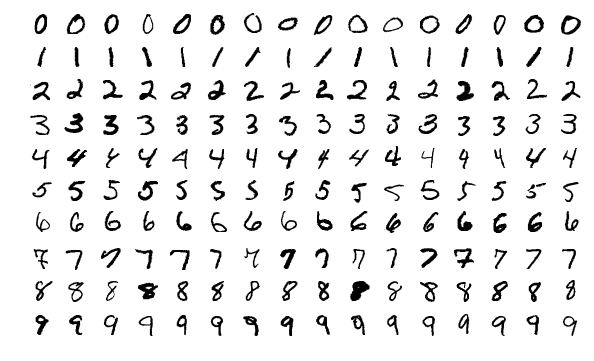
\includegraphics[width=\linewidth]{MnistExamples.png}
						\caption{Příklad obrázků z datasetu MNIST\\TODO(\url{https://upload.wikimedia.org/wikipedia/commons/2/27/MnistExamples.png})}
						\label{fig:MNIST}
					\end{figure}
					
					Tuto databázi jsem použil pro první testování BasicNeuralNetwork, jelikož má pro první testování dostačující velikost. Pro pozdější testování využívám převážně EMNIST.
				\subsection{Databáze EMNIST}
					\uv{Databáze MNIST se stala standardem pro učení umělého vidění. Databáze MNIST je odvozená z databáze NIST Special Database 19, která obsahuje ručně psané číslice a velká i malá písmena. EMNIST (Extended MNIST), varianta celé databáze NIST, přebírá uspořádání z databáze MNIST\footnote{Má však prohozené řádky a sloupce obrázků.}.} \parencite[přeloženo]{article:EMNIST}
					
					Tato databáze obsahuje více příkladů než MNIST, navíc obsahuje i sety s písmeny, proto jsem po prvních pokusech s MNIST přešel na tuto databázi.

		\chapter{Používání knihovny}
			\section{Nastavování hodnot}
				Neuronová síť má mnoho hodnot, které lze nastavit, z mého testování knihovny vyplývá, že minimálně na rozpoznávání čísel:
				\begin{itemize}
					\item Learning rate je třeba nastavit na cca 0.1 a pomalu snižovat.
					\item Počet skrytá vrstva musí být právě 1 (2 už se nenaučí propojit vstup s výstupem a bez skryté vrstvy vůbec nefunguje). Pokud byste potřebovali učit síť s více skrytými vrstvami, musíte nastavit learning rate na daleko nižší hodnotu.
					\item Počet neuronů ve skryté vrstvě je hodně variabilní, ideálně mezi hodnotami 100 a 300.
					\item Jako aktivační funkce stačí třeba sigmoida, jiné jsem nepoužíval.
				\end{itemize}


	\appendix
	\addcontentsline{toc}{part}{Apendix}
	
	\chapter*{Závěr}
	
		Povedlo se mi implementovat neuronovou síť do takové míry, aby byla schopna rozeznávat číslice (TODO(znaky/číslice)) (ukázka je na stránkách \url{moznabude.cz}). Dále bych mohl pokračovat například implementováním lepšího ukládání do souboru (ukládání typu \verb!Double! jako textového řetězce není moc efektivní), implementování nějakých genetických algoritmů, či naprogramování konvoluční sítě tak, aby filtry mohly pracovat $n$ rozměrně.
	
	\nocite{*}
    \printbibliography					% Vytvoří seznam literatury
	\addcontentsline{toc}{chapter}{Bibliografie}
    \printglossary[title={Slovníček pojmů}]	% Vytvoří seznam zkratek
    \listoffigures						% Vytvoří seznam obrázků
    %\listoftables						% Vytvoří seznam tabulek
    
    \begin{prilohy}
    	\pitem{Fotky z pokusů}
    	\eitem{Vlastní program}
    	\eitem{Dokumentace}
    	\eitem{Testovací data}
    \end{prilohy}
\end{document}